% lecture4_ro.tex -- GENERATED by build_L4.py from L4_numbers.json; do not edit by hand.
\documentclass[10pt,aspectratio=169,t]{beamer}
% =============================================================================
% emqa_preamble.tex -- shared Beamer preamble of Energy Markets Quantitative Analysis (EMQA)
% Used by every lecture: lectures/Lk/lecturek.tex does
%   \documentclass[10pt,aspectratio=169,t]{beamer}
%   % =============================================================================
% emqa_preamble.tex -- shared Beamer preamble of Energy Markets Quantitative Analysis (EMQA)
% Used by every lecture: lectures/Lk/lecturek.tex does
%   \documentclass[10pt,aspectratio=169,t]{beamer}
%   % =============================================================================
% emqa_preamble.tex -- shared Beamer preamble of Energy Markets Quantitative Analysis (EMQA)
% Used by every lecture: lectures/Lk/lecturek.tex does
%   \documentclass[10pt,aspectratio=169,t]{beamer}
%   \input{../common/emqa_preamble}
%   \emqalecture{k}{Lecture title}
% Logos live in lectures/common/logos/, charts in lectures/Lk/charts/.
% Do NOT add \hfuzz / \vfuzz / \hbadness here: overfull boxes must be fixed, not hidden.
% =============================================================================

\usetheme{default}
\setbeamersize{text margin left=7mm, text margin right=7mm}

% ---------------------------------------------------------------- packages
\usepackage[utf8]{inputenc}
\usepackage[T1]{fontenc}
\usepackage{lmodern}
\usepackage{amsmath, amssymb}
\usepackage{mathtools}
\usepackage{bm}
\usepackage{tikz}
\usetikzlibrary{arrows.meta, positioning, calc, shapes.misc}
\usepackage{booktabs}
\usepackage{array}
\usepackage{graphicx}
\usepackage{colortbl}
\usepackage{xcolor}
\usepackage{multicol}
\hypersetup{colorlinks=true, linkcolor=MainBlue, urlcolor=MainBlue, citecolor=MainBlue}
\graphicspath{{../common/logos/}}   % charts are included with their language folder: charts/en/, charts/ro/

% ---------------------------------------------------------------- colours
\definecolor{MainBlue}{RGB}{26, 58, 110}
\definecolor{IDAred}{RGB}{205, 0, 0}
\definecolor{DarkGray}{RGB}{51, 51, 51}
\definecolor{FooterGray}{RGB}{100, 100, 100}
\definecolor{BlockGray}{RGB}{236, 238, 242}
\definecolor{KeynoteGray}{RGB}{218, 218, 218}
\definecolor{Crimson}{RGB}{190, 40, 50}
\definecolor{Forest}{RGB}{30, 110, 50}
\definecolor{Bitter}{RGB}{214, 150, 20}
% chart palette (same hex values as lectures/common/emqa_plot.py)
\definecolor{SerRO}{HTML}{2A78D6}
\definecolor{SerDE}{HTML}{EB6834}
\definecolor{SerHU}{HTML}{1BAF7A}
\definecolor{SerBG}{HTML}{EDA100}

\setbeamertemplate{background}{%
  \begin{tikzpicture}[remember picture, overlay]
    \shade[shading=axis, shading angle=315, top color=white, bottom color=KeynoteGray]
      (current page.south west) rectangle (current page.north east);
  \end{tikzpicture}}
\setbeamercolor{background canvas}{bg=}
\setbeamercolor{structure}{fg=MainBlue}
\setbeamercolor{normal text}{fg=DarkGray}
\setbeamercolor{title}{fg=IDAred}
\setbeamercolor{frametitle}{fg=IDAred, bg=}
\setbeamercolor{block title}{bg=MainBlue, fg=white}
\setbeamercolor{block body}{bg=BlockGray, fg=DarkGray}
\setbeamercolor{block title alerted}{bg=Crimson, fg=white}
\setbeamercolor{block body alerted}{bg=Crimson!7, fg=DarkGray}
\setbeamercolor{block title example}{bg=Forest, fg=white}
\setbeamercolor{block body example}{bg=Forest!7, fg=DarkGray}
\setbeamercolor{item}{fg=MainBlue}
\setbeamerfont{frametitle}{size=\large, series=\bfseries}
\setbeamerfont{block title}{size=\small, series=\bfseries}
\setbeamertemplate{blocks}[rounded][shadow=false]
\setbeamertemplate{itemize item}{\color{MainBlue}$\boxdot$}
\setbeamertemplate{itemize subitem}{\color{MainBlue}\scriptsize$\blacktriangleright$}
% compact two-level lists: level 1 = main point, level 2 = details (no text outside bullets)
\setbeamerfont{itemize/enumerate subbody}{size=\footnotesize}
\setlength{\leftmargini}{1.1em}
\setlength{\leftmarginii}{1.1em}
\setbeamertemplate{itemize/enumerate body begin}{\setlength{\topsep}{0pt}\setlength{\partopsep}{0pt}\setlength{\parskip}{0pt}}
\setbeamertemplate{itemize/enumerate subbody begin}{\setlength{\topsep}{0pt}\setlength{\partopsep}{0pt}\setlength{\itemsep}{0pt}\vspace{-0.4ex}}

\setbeamertemplate{enumerate item}{\color{MainBlue}\insertenumlabel.}
\setlength{\leftmargini}{1.3em}
\setlength{\leftmarginii}{1.2em}
\setbeamertemplate{navigation symbols}{}
\setbeamertemplate{section in toc}{\color{MainBlue}$\blacktriangleright$~\inserttocsection}
\setbeamertemplate{caption}{\raggedright\insertcaption\par}
% frame subtitle = precise citation line under the claim title (Weron style)
\setbeamerfont{framesubtitle}{size=\footnotesize}
\setbeamercolor{framesubtitle}{fg=FooterGray}
% outline that reappears at every section with the current section highlighted
\setbeamertemplate{section in toc shaded}[default][35]
\setbeamertemplate{subsection in toc shaded}[default][35]
\setbeamertemplate{subsection in toc}{\leavevmode\leftskip=2.2em\color{DarkGray}\small\inserttocsubsection\par}
\AtBeginSection[]{{\begin{frame}{\txtoutline}\vspace{2mm}\small
  \tableofcontents[currentsection,hideothersubsections]\end{frame}}}

% ---------------------------------------------------------------- head and foot
\setbeamertemplate{headline}{%
  \vskip10pt%
  \hbox to \paperwidth{\hskip0.5cm%
    {\small\color{FooterGray}\renewcommand{\hyperlink}[2]{##2}\insertsectionhead}%
    \hfill\textcolor{FooterGray}{\small\insertframenumber}\hskip0.5cm}%
  \vskip4pt{\color{FooterGray}\hrule height 0.4pt}}
% footer as in the other courses (MFM, SFM): course name on the left, small sparkline on the right
\setbeamertemplate{footline}{%
  {\color{FooterGray}\hrule height 0.4pt}\vskip4pt%
  \hbox to \paperwidth{\hskip0.5cm%
    \textcolor{FooterGray}{\small\txtcourse}%
    \hfill\raisebox{-0.1em}{\begin{tikzpicture}[x=0.08em, y=0.08em, line width=0.4pt]
      \draw[FooterGray] (0,3) -- (1,4) -- (2,3.5) -- (3,5) -- (4,4) -- (5,6) -- (6,5.5) -- (7,4) -- (8,5) -- (9,7) -- (10,6) -- (11,5) -- (12,6.5) -- (13,8) -- (14,7) -- (15,6) -- (16,7.5) -- (17,9) -- (18,8) -- (19,7) -- (20,8.5) -- (21,10) -- (22,9) -- (23,8) -- (24,9.5);
    \end{tikzpicture}}\hskip0.5cm}%
  \vskip6pt}

% ---------------------------------------------------------------- title page
\defbeamertemplate*{title page}{emqa}[1][]{%
  \vspace{0.15cm}
  \begin{center}
    \href{https://www.ase.ro}{
\includegraphics[height=0.9cm]{ase_logo.png}}\hspace{0.3cm}%
    \href{https://ipe.ro/new}{
\includegraphics[height=0.9cm]{acad_logo.png}}\hspace{0.3cm}%
    \href{https://theida.net}{
\includegraphics[height=0.9cm]{ida_logo.png}}\hspace{0.3cm}%
    \href{https://blockchain-research-center.com}{
\includegraphics[height=0.9cm]{brc_logo.png}}\hspace{0.3cm}%
    \href{https://www.ai4efin.ase.ro}{
\includegraphics[height=0.9cm]{ai4efin_logo.png}}\hspace{0.3cm}%
    \href{https://www.digital-finance-msca.com}{
\includegraphics[height=0.9cm]{msca_logo.png}}%
  \end{center}
  \vspace{0.45cm}
  \begin{center}
    \begin{minipage}{0.1\textwidth}\centering
      \href{https://quantlet.com}{
\includegraphics[height=0.9cm]{ql_logo.png}}\end{minipage}%
    \begin{minipage}{0.78\textwidth}\centering
      {\Large\bfseries\usebeamercolor[fg]{title}\inserttitle}\par\vspace{0.25cm}
      {\large\usebeamercolor[fg]{title}\insertsubtitle}\end{minipage}%
    \begin{minipage}{0.1\textwidth}\centering
      \href{https://quantinar.com}{
\includegraphics[height=0.9cm]{qr_logo.png}}\end{minipage}
  \end{center}
  \vfill
  \hspace{0.4cm}{\bfseries\insertauthor}\par\vspace{0.12cm}
  \hspace{0.4cm}\begin{minipage}[t]{0.92\textwidth}\raggedright\footnotesize\insertinstitute\end{minipage}
  \par\vspace{0.4cm}}

% ---------------------------------------------------------------- lecture metadata
\newcommand{\emqashort}{}
\newcommand{\emqanb}{notebooks}
\newcommand{\emqarepo}{https://github.com/danpele/EMQA/tree/main}
% language-dependent labels (English default; \emqaromanian switches to Romanian, call it before \emqalecture)
\newcommand{\txtcourse}{Energy Markets Quantitative Analysis}
\newcommand{\txtlecture}{Lecture}
\newcommand{\txtoutline}{Outline}
\newcommand{\txtintuition}{In one sentence:}
\newcommand{\txtjob}{In practice:}
\newcommand{\txttry}{Experiment yourself:}
\newcommand{\txtwhere}{where}
\newcommand{\txtsim}{SIMULATED DATA (teaching illustration)}
\newcommand{\txtnbsuffix}{}
\newcommand{\txtinstitute}{Bucharest University of Economic Studies, Department of Statistics and Econometrics\\
    Romanian Academy, Institute for Economic Forecasting\\
    IDA Institute Digital Assets \textbullet\ AI4EFin \textbullet\ MSCA Digital Finance}
\newcommand{\emqaromanian}{%
  \renewcommand{\txtcourse}{Analiza cantitativă a piețelor de energie}%
  \renewcommand{\txtlecture}{Cursul}%
  \renewcommand{\txtoutline}{Cuprins}%
  \renewcommand{\txtintuition}{Pe scurt:}%
  \renewcommand{\txtjob}{În practică:}%
  \renewcommand{\txttry}{Exercițiu practic:}%
  \renewcommand{\txtwhere}{unde}%
  \renewcommand{\txtsim}{DATE SIMULATE (doar pentru ilustrare)}%
  \renewcommand{\txtnbsuffix}{\string_ro}%
  \renewcommand{\txtinstitute}{Academia de Studii Economice din București, Departamentul de Statistică și Econometrie\\
    Academia Română, Institutul de Prognoză Economică\\
    IDA Institute Digital Assets \textbullet\ AI4EFin \textbullet\ MSCA Digital Finance}}
\newcommand{\emqalecture}[2]{%
  \renewcommand{\emqashort}{\txtlecture\ #1}%
  \renewcommand{\emqanb}{notebooks/L#1\string_notebook\txtnbsuffix.ipynb}%
  \title[EMQA]{\txtcourse}%
  \subtitle{\txtlecture\ #1: #2}%
  \author{Prof.\ dr.\ Daniel Traian PELE}%
  \institute{\txtinstitute}%
  \date{}}

% ---------------------------------------------------------------- teaching blocks (MBA clarity rule)
% \intuition{one plain sentence}  ->  formula with every symbol defined  ->  real-data example  ->  \manager{one line}
\newcommand{\intuition}[1]{\begin{itemize}\item {\color{MainBlue}\textbf{\txtintuition}}~#1\end{itemize}\vspace{0.6mm}}
\newcommand{\manager}[1]{\colorbox{Forest!10}{\parbox{\dimexpr\linewidth-2\fboxsep\relax}{\footnotesize
  \begin{itemize}\setlength{\itemsep}{0pt}\item \textbf{\color{Forest}\txtjob}~#1\end{itemize}}}}
% Experiment yourself: pointer to the matching notebook section
\newcommand{\tryit}[1]{{\scriptsize\href{\emqarepo/\emqanb}{%
  \raisebox{-0.15em}{
\includegraphics[height=0.85em]{ql_logo.png}}\,\textbf{\txttry}~\color{MainBlue}#1}}}
% bottom row: manager line (left) + experiment pointer (right), pinned to the bottom of the frame
\newcommand{\bottomrow}[2]{\par\vfill\noindent\begin{minipage}[b]{0.72\linewidth}#1\end{minipage}\hfill
  \begin{minipage}[b]{0.26\linewidth}\raggedleft #2\end{minipage}\par\vspace{0.5mm}}
\newcommand{\where}[1]{{\footnotesize\textbf{\txtwhere}~#1\par}}

% ---------------------------------------------------------------- helpers
% chart source line under a figure: \chartsource{Source ...; period ...}
\newcommand{\chartsource}[1]{\par\vspace{1pt}{\scriptsize\color{FooterGray}#1\par}}
% link to code: \quantlet{label}{path inside the repo}
\newcommand{\quantlet}[2]{\par\vspace{1pt}\hfill\href{\emqarepo/#2}{%
  \raisebox{-0.15em}{
\includegraphics[height=0.75em]{ql_logo.png}}\textcolor{MainBlue}{\scriptsize\ #1}}}
\newcommand{\simlabel}{\colorbox{Crimson!12}{\scriptsize\bfseries\color{Crimson}\txtsim}}
\newcommand{\E}{\mathbb{E}}
\newcommand{\Var}{\operatorname{Var}}
\newcommand{\Cov}{\operatorname{Cov}}
\newcommand{\Corr}{\operatorname{Corr}}
\newcommand{\asinh}{\operatorname{asinh}}
\newcommand{\iid}{\overset{\text{i.i.d.}}{\sim}}
\newcommand{\EUR}{EUR}

%   \emqalecture{k}{Lecture title}
% Logos live in lectures/common/logos/, charts in lectures/Lk/charts/.
% Do NOT add \hfuzz / \vfuzz / \hbadness here: overfull boxes must be fixed, not hidden.
% =============================================================================

\usetheme{default}
\setbeamersize{text margin left=7mm, text margin right=7mm}

% ---------------------------------------------------------------- packages
\usepackage[utf8]{inputenc}
\usepackage[T1]{fontenc}
\usepackage{lmodern}
\usepackage{amsmath, amssymb}
\usepackage{mathtools}
\usepackage{bm}
\usepackage{tikz}
\usetikzlibrary{arrows.meta, positioning, calc, shapes.misc}
\usepackage{booktabs}
\usepackage{array}
\usepackage{graphicx}
\usepackage{colortbl}
\usepackage{xcolor}
\usepackage{multicol}
\hypersetup{colorlinks=true, linkcolor=MainBlue, urlcolor=MainBlue, citecolor=MainBlue}
\graphicspath{{../common/logos/}}   % charts are included with their language folder: charts/en/, charts/ro/

% ---------------------------------------------------------------- colours
\definecolor{MainBlue}{RGB}{26, 58, 110}
\definecolor{IDAred}{RGB}{205, 0, 0}
\definecolor{DarkGray}{RGB}{51, 51, 51}
\definecolor{FooterGray}{RGB}{100, 100, 100}
\definecolor{BlockGray}{RGB}{236, 238, 242}
\definecolor{KeynoteGray}{RGB}{218, 218, 218}
\definecolor{Crimson}{RGB}{190, 40, 50}
\definecolor{Forest}{RGB}{30, 110, 50}
\definecolor{Bitter}{RGB}{214, 150, 20}
% chart palette (same hex values as lectures/common/emqa_plot.py)
\definecolor{SerRO}{HTML}{2A78D6}
\definecolor{SerDE}{HTML}{EB6834}
\definecolor{SerHU}{HTML}{1BAF7A}
\definecolor{SerBG}{HTML}{EDA100}

\setbeamertemplate{background}{%
  \begin{tikzpicture}[remember picture, overlay]
    \shade[shading=axis, shading angle=315, top color=white, bottom color=KeynoteGray]
      (current page.south west) rectangle (current page.north east);
  \end{tikzpicture}}
\setbeamercolor{background canvas}{bg=}
\setbeamercolor{structure}{fg=MainBlue}
\setbeamercolor{normal text}{fg=DarkGray}
\setbeamercolor{title}{fg=IDAred}
\setbeamercolor{frametitle}{fg=IDAred, bg=}
\setbeamercolor{block title}{bg=MainBlue, fg=white}
\setbeamercolor{block body}{bg=BlockGray, fg=DarkGray}
\setbeamercolor{block title alerted}{bg=Crimson, fg=white}
\setbeamercolor{block body alerted}{bg=Crimson!7, fg=DarkGray}
\setbeamercolor{block title example}{bg=Forest, fg=white}
\setbeamercolor{block body example}{bg=Forest!7, fg=DarkGray}
\setbeamercolor{item}{fg=MainBlue}
\setbeamerfont{frametitle}{size=\large, series=\bfseries}
\setbeamerfont{block title}{size=\small, series=\bfseries}
\setbeamertemplate{blocks}[rounded][shadow=false]
\setbeamertemplate{itemize item}{\color{MainBlue}$\boxdot$}
\setbeamertemplate{itemize subitem}{\color{MainBlue}\scriptsize$\blacktriangleright$}
% compact two-level lists: level 1 = main point, level 2 = details (no text outside bullets)
\setbeamerfont{itemize/enumerate subbody}{size=\footnotesize}
\setlength{\leftmargini}{1.1em}
\setlength{\leftmarginii}{1.1em}
\setbeamertemplate{itemize/enumerate body begin}{\setlength{\topsep}{0pt}\setlength{\partopsep}{0pt}\setlength{\parskip}{0pt}}
\setbeamertemplate{itemize/enumerate subbody begin}{\setlength{\topsep}{0pt}\setlength{\partopsep}{0pt}\setlength{\itemsep}{0pt}\vspace{-0.4ex}}

\setbeamertemplate{enumerate item}{\color{MainBlue}\insertenumlabel.}
\setlength{\leftmargini}{1.3em}
\setlength{\leftmarginii}{1.2em}
\setbeamertemplate{navigation symbols}{}
\setbeamertemplate{section in toc}{\color{MainBlue}$\blacktriangleright$~\inserttocsection}
\setbeamertemplate{caption}{\raggedright\insertcaption\par}
% frame subtitle = precise citation line under the claim title (Weron style)
\setbeamerfont{framesubtitle}{size=\footnotesize}
\setbeamercolor{framesubtitle}{fg=FooterGray}
% outline that reappears at every section with the current section highlighted
\setbeamertemplate{section in toc shaded}[default][35]
\setbeamertemplate{subsection in toc shaded}[default][35]
\setbeamertemplate{subsection in toc}{\leavevmode\leftskip=2.2em\color{DarkGray}\small\inserttocsubsection\par}
\AtBeginSection[]{{\begin{frame}{\txtoutline}\vspace{2mm}\small
  \tableofcontents[currentsection,hideothersubsections]\end{frame}}}

% ---------------------------------------------------------------- head and foot
\setbeamertemplate{headline}{%
  \vskip10pt%
  \hbox to \paperwidth{\hskip0.5cm%
    {\small\color{FooterGray}\renewcommand{\hyperlink}[2]{##2}\insertsectionhead}%
    \hfill\textcolor{FooterGray}{\small\insertframenumber}\hskip0.5cm}%
  \vskip4pt{\color{FooterGray}\hrule height 0.4pt}}
% footer as in the other courses (MFM, SFM): course name on the left, small sparkline on the right
\setbeamertemplate{footline}{%
  {\color{FooterGray}\hrule height 0.4pt}\vskip4pt%
  \hbox to \paperwidth{\hskip0.5cm%
    \textcolor{FooterGray}{\small\txtcourse}%
    \hfill\raisebox{-0.1em}{\begin{tikzpicture}[x=0.08em, y=0.08em, line width=0.4pt]
      \draw[FooterGray] (0,3) -- (1,4) -- (2,3.5) -- (3,5) -- (4,4) -- (5,6) -- (6,5.5) -- (7,4) -- (8,5) -- (9,7) -- (10,6) -- (11,5) -- (12,6.5) -- (13,8) -- (14,7) -- (15,6) -- (16,7.5) -- (17,9) -- (18,8) -- (19,7) -- (20,8.5) -- (21,10) -- (22,9) -- (23,8) -- (24,9.5);
    \end{tikzpicture}}\hskip0.5cm}%
  \vskip6pt}

% ---------------------------------------------------------------- title page
\defbeamertemplate*{title page}{emqa}[1][]{%
  \vspace{0.15cm}
  \begin{center}
    \href{https://www.ase.ro}{
\includegraphics[height=0.9cm]{ase_logo.png}}\hspace{0.3cm}%
    \href{https://ipe.ro/new}{
\includegraphics[height=0.9cm]{acad_logo.png}}\hspace{0.3cm}%
    \href{https://theida.net}{
\includegraphics[height=0.9cm]{ida_logo.png}}\hspace{0.3cm}%
    \href{https://blockchain-research-center.com}{
\includegraphics[height=0.9cm]{brc_logo.png}}\hspace{0.3cm}%
    \href{https://www.ai4efin.ase.ro}{
\includegraphics[height=0.9cm]{ai4efin_logo.png}}\hspace{0.3cm}%
    \href{https://www.digital-finance-msca.com}{
\includegraphics[height=0.9cm]{msca_logo.png}}%
  \end{center}
  \vspace{0.45cm}
  \begin{center}
    \begin{minipage}{0.1\textwidth}\centering
      \href{https://quantlet.com}{
\includegraphics[height=0.9cm]{ql_logo.png}}\end{minipage}%
    \begin{minipage}{0.78\textwidth}\centering
      {\Large\bfseries\usebeamercolor[fg]{title}\inserttitle}\par\vspace{0.25cm}
      {\large\usebeamercolor[fg]{title}\insertsubtitle}\end{minipage}%
    \begin{minipage}{0.1\textwidth}\centering
      \href{https://quantinar.com}{
\includegraphics[height=0.9cm]{qr_logo.png}}\end{minipage}
  \end{center}
  \vfill
  \hspace{0.4cm}{\bfseries\insertauthor}\par\vspace{0.12cm}
  \hspace{0.4cm}\begin{minipage}[t]{0.92\textwidth}\raggedright\footnotesize\insertinstitute\end{minipage}
  \par\vspace{0.4cm}}

% ---------------------------------------------------------------- lecture metadata
\newcommand{\emqashort}{}
\newcommand{\emqanb}{notebooks}
\newcommand{\emqarepo}{https://github.com/danpele/EMQA/tree/main}
% language-dependent labels (English default; \emqaromanian switches to Romanian, call it before \emqalecture)
\newcommand{\txtcourse}{Energy Markets Quantitative Analysis}
\newcommand{\txtlecture}{Lecture}
\newcommand{\txtoutline}{Outline}
\newcommand{\txtintuition}{In one sentence:}
\newcommand{\txtjob}{In practice:}
\newcommand{\txttry}{Experiment yourself:}
\newcommand{\txtwhere}{where}
\newcommand{\txtsim}{SIMULATED DATA (teaching illustration)}
\newcommand{\txtnbsuffix}{}
\newcommand{\txtinstitute}{Bucharest University of Economic Studies, Department of Statistics and Econometrics\\
    Romanian Academy, Institute for Economic Forecasting\\
    IDA Institute Digital Assets \textbullet\ AI4EFin \textbullet\ MSCA Digital Finance}
\newcommand{\emqaromanian}{%
  \renewcommand{\txtcourse}{Analiza cantitativă a piețelor de energie}%
  \renewcommand{\txtlecture}{Cursul}%
  \renewcommand{\txtoutline}{Cuprins}%
  \renewcommand{\txtintuition}{Pe scurt:}%
  \renewcommand{\txtjob}{În practică:}%
  \renewcommand{\txttry}{Exercițiu practic:}%
  \renewcommand{\txtwhere}{unde}%
  \renewcommand{\txtsim}{DATE SIMULATE (doar pentru ilustrare)}%
  \renewcommand{\txtnbsuffix}{\string_ro}%
  \renewcommand{\txtinstitute}{Academia de Studii Economice din București, Departamentul de Statistică și Econometrie\\
    Academia Română, Institutul de Prognoză Economică\\
    IDA Institute Digital Assets \textbullet\ AI4EFin \textbullet\ MSCA Digital Finance}}
\newcommand{\emqalecture}[2]{%
  \renewcommand{\emqashort}{\txtlecture\ #1}%
  \renewcommand{\emqanb}{notebooks/L#1\string_notebook\txtnbsuffix.ipynb}%
  \title[EMQA]{\txtcourse}%
  \subtitle{\txtlecture\ #1: #2}%
  \author{Prof.\ dr.\ Daniel Traian PELE}%
  \institute{\txtinstitute}%
  \date{}}

% ---------------------------------------------------------------- teaching blocks (MBA clarity rule)
% \intuition{one plain sentence}  ->  formula with every symbol defined  ->  real-data example  ->  \manager{one line}
\newcommand{\intuition}[1]{\begin{itemize}\item {\color{MainBlue}\textbf{\txtintuition}}~#1\end{itemize}\vspace{0.6mm}}
\newcommand{\manager}[1]{\colorbox{Forest!10}{\parbox{\dimexpr\linewidth-2\fboxsep\relax}{\footnotesize
  \begin{itemize}\setlength{\itemsep}{0pt}\item \textbf{\color{Forest}\txtjob}~#1\end{itemize}}}}
% Experiment yourself: pointer to the matching notebook section
\newcommand{\tryit}[1]{{\scriptsize\href{\emqarepo/\emqanb}{%
  \raisebox{-0.15em}{
\includegraphics[height=0.85em]{ql_logo.png}}\,\textbf{\txttry}~\color{MainBlue}#1}}}
% bottom row: manager line (left) + experiment pointer (right), pinned to the bottom of the frame
\newcommand{\bottomrow}[2]{\par\vfill\noindent\begin{minipage}[b]{0.72\linewidth}#1\end{minipage}\hfill
  \begin{minipage}[b]{0.26\linewidth}\raggedleft #2\end{minipage}\par\vspace{0.5mm}}
\newcommand{\where}[1]{{\footnotesize\textbf{\txtwhere}~#1\par}}

% ---------------------------------------------------------------- helpers
% chart source line under a figure: \chartsource{Source ...; period ...}
\newcommand{\chartsource}[1]{\par\vspace{1pt}{\scriptsize\color{FooterGray}#1\par}}
% link to code: \quantlet{label}{path inside the repo}
\newcommand{\quantlet}[2]{\par\vspace{1pt}\hfill\href{\emqarepo/#2}{%
  \raisebox{-0.15em}{
\includegraphics[height=0.75em]{ql_logo.png}}\textcolor{MainBlue}{\scriptsize\ #1}}}
\newcommand{\simlabel}{\colorbox{Crimson!12}{\scriptsize\bfseries\color{Crimson}\txtsim}}
\newcommand{\E}{\mathbb{E}}
\newcommand{\Var}{\operatorname{Var}}
\newcommand{\Cov}{\operatorname{Cov}}
\newcommand{\Corr}{\operatorname{Corr}}
\newcommand{\asinh}{\operatorname{asinh}}
\newcommand{\iid}{\overset{\text{i.i.d.}}{\sim}}
\newcommand{\EUR}{EUR}

%   \emqalecture{k}{Lecture title}
% Logos live in lectures/common/logos/, charts in lectures/Lk/charts/.
% Do NOT add \hfuzz / \vfuzz / \hbadness here: overfull boxes must be fixed, not hidden.
% =============================================================================

\usetheme{default}
\setbeamersize{text margin left=7mm, text margin right=7mm}

% ---------------------------------------------------------------- packages
\usepackage[utf8]{inputenc}
\usepackage[T1]{fontenc}
\usepackage{lmodern}
\usepackage{amsmath, amssymb}
\usepackage{mathtools}
\usepackage{bm}
\usepackage{tikz}
\usetikzlibrary{arrows.meta, positioning, calc, shapes.misc}
\usepackage{booktabs}
\usepackage{array}
\usepackage{graphicx}
\usepackage{colortbl}
\usepackage{xcolor}
\usepackage{multicol}
\hypersetup{colorlinks=true, linkcolor=MainBlue, urlcolor=MainBlue, citecolor=MainBlue}
\graphicspath{{../common/logos/}}   % charts are included with their language folder: charts/en/, charts/ro/

% ---------------------------------------------------------------- colours
\definecolor{MainBlue}{RGB}{26, 58, 110}
\definecolor{IDAred}{RGB}{205, 0, 0}
\definecolor{DarkGray}{RGB}{51, 51, 51}
\definecolor{FooterGray}{RGB}{100, 100, 100}
\definecolor{BlockGray}{RGB}{236, 238, 242}
\definecolor{KeynoteGray}{RGB}{218, 218, 218}
\definecolor{Crimson}{RGB}{190, 40, 50}
\definecolor{Forest}{RGB}{30, 110, 50}
\definecolor{Bitter}{RGB}{214, 150, 20}
% chart palette (same hex values as lectures/common/emqa_plot.py)
\definecolor{SerRO}{HTML}{2A78D6}
\definecolor{SerDE}{HTML}{EB6834}
\definecolor{SerHU}{HTML}{1BAF7A}
\definecolor{SerBG}{HTML}{EDA100}

\setbeamertemplate{background}{%
  \begin{tikzpicture}[remember picture, overlay]
    \shade[shading=axis, shading angle=315, top color=white, bottom color=KeynoteGray]
      (current page.south west) rectangle (current page.north east);
  \end{tikzpicture}}
\setbeamercolor{background canvas}{bg=}
\setbeamercolor{structure}{fg=MainBlue}
\setbeamercolor{normal text}{fg=DarkGray}
\setbeamercolor{title}{fg=IDAred}
\setbeamercolor{frametitle}{fg=IDAred, bg=}
\setbeamercolor{block title}{bg=MainBlue, fg=white}
\setbeamercolor{block body}{bg=BlockGray, fg=DarkGray}
\setbeamercolor{block title alerted}{bg=Crimson, fg=white}
\setbeamercolor{block body alerted}{bg=Crimson!7, fg=DarkGray}
\setbeamercolor{block title example}{bg=Forest, fg=white}
\setbeamercolor{block body example}{bg=Forest!7, fg=DarkGray}
\setbeamercolor{item}{fg=MainBlue}
\setbeamerfont{frametitle}{size=\large, series=\bfseries}
\setbeamerfont{block title}{size=\small, series=\bfseries}
\setbeamertemplate{blocks}[rounded][shadow=false]
\setbeamertemplate{itemize item}{\color{MainBlue}$\boxdot$}
\setbeamertemplate{itemize subitem}{\color{MainBlue}\scriptsize$\blacktriangleright$}
% compact two-level lists: level 1 = main point, level 2 = details (no text outside bullets)
\setbeamerfont{itemize/enumerate subbody}{size=\footnotesize}
\setlength{\leftmargini}{1.1em}
\setlength{\leftmarginii}{1.1em}
\setbeamertemplate{itemize/enumerate body begin}{\setlength{\topsep}{0pt}\setlength{\partopsep}{0pt}\setlength{\parskip}{0pt}}
\setbeamertemplate{itemize/enumerate subbody begin}{\setlength{\topsep}{0pt}\setlength{\partopsep}{0pt}\setlength{\itemsep}{0pt}\vspace{-0.4ex}}

\setbeamertemplate{enumerate item}{\color{MainBlue}\insertenumlabel.}
\setlength{\leftmargini}{1.3em}
\setlength{\leftmarginii}{1.2em}
\setbeamertemplate{navigation symbols}{}
\setbeamertemplate{section in toc}{\color{MainBlue}$\blacktriangleright$~\inserttocsection}
\setbeamertemplate{caption}{\raggedright\insertcaption\par}
% frame subtitle = precise citation line under the claim title (Weron style)
\setbeamerfont{framesubtitle}{size=\footnotesize}
\setbeamercolor{framesubtitle}{fg=FooterGray}
% outline that reappears at every section with the current section highlighted
\setbeamertemplate{section in toc shaded}[default][35]
\setbeamertemplate{subsection in toc shaded}[default][35]
\setbeamertemplate{subsection in toc}{\leavevmode\leftskip=2.2em\color{DarkGray}\small\inserttocsubsection\par}
\AtBeginSection[]{{\begin{frame}{\txtoutline}\vspace{2mm}\small
  \tableofcontents[currentsection,hideothersubsections]\end{frame}}}

% ---------------------------------------------------------------- head and foot
\setbeamertemplate{headline}{%
  \vskip10pt%
  \hbox to \paperwidth{\hskip0.5cm%
    {\small\color{FooterGray}\renewcommand{\hyperlink}[2]{##2}\insertsectionhead}%
    \hfill\textcolor{FooterGray}{\small\insertframenumber}\hskip0.5cm}%
  \vskip4pt{\color{FooterGray}\hrule height 0.4pt}}
% footer as in the other courses (MFM, SFM): course name on the left, small sparkline on the right
\setbeamertemplate{footline}{%
  {\color{FooterGray}\hrule height 0.4pt}\vskip4pt%
  \hbox to \paperwidth{\hskip0.5cm%
    \textcolor{FooterGray}{\small\txtcourse}%
    \hfill\raisebox{-0.1em}{\begin{tikzpicture}[x=0.08em, y=0.08em, line width=0.4pt]
      \draw[FooterGray] (0,3) -- (1,4) -- (2,3.5) -- (3,5) -- (4,4) -- (5,6) -- (6,5.5) -- (7,4) -- (8,5) -- (9,7) -- (10,6) -- (11,5) -- (12,6.5) -- (13,8) -- (14,7) -- (15,6) -- (16,7.5) -- (17,9) -- (18,8) -- (19,7) -- (20,8.5) -- (21,10) -- (22,9) -- (23,8) -- (24,9.5);
    \end{tikzpicture}}\hskip0.5cm}%
  \vskip6pt}

% ---------------------------------------------------------------- title page
\defbeamertemplate*{title page}{emqa}[1][]{%
  \vspace{0.15cm}
  \begin{center}
    \href{https://www.ase.ro}{
\includegraphics[height=0.9cm]{ase_logo.png}}\hspace{0.3cm}%
    \href{https://ipe.ro/new}{
\includegraphics[height=0.9cm]{acad_logo.png}}\hspace{0.3cm}%
    \href{https://theida.net}{
\includegraphics[height=0.9cm]{ida_logo.png}}\hspace{0.3cm}%
    \href{https://blockchain-research-center.com}{
\includegraphics[height=0.9cm]{brc_logo.png}}\hspace{0.3cm}%
    \href{https://www.ai4efin.ase.ro}{
\includegraphics[height=0.9cm]{ai4efin_logo.png}}\hspace{0.3cm}%
    \href{https://www.digital-finance-msca.com}{
\includegraphics[height=0.9cm]{msca_logo.png}}%
  \end{center}
  \vspace{0.45cm}
  \begin{center}
    \begin{minipage}{0.1\textwidth}\centering
      \href{https://quantlet.com}{
\includegraphics[height=0.9cm]{ql_logo.png}}\end{minipage}%
    \begin{minipage}{0.78\textwidth}\centering
      {\Large\bfseries\usebeamercolor[fg]{title}\inserttitle}\par\vspace{0.25cm}
      {\large\usebeamercolor[fg]{title}\insertsubtitle}\end{minipage}%
    \begin{minipage}{0.1\textwidth}\centering
      \href{https://quantinar.com}{
\includegraphics[height=0.9cm]{qr_logo.png}}\end{minipage}
  \end{center}
  \vfill
  \hspace{0.4cm}{\bfseries\insertauthor}\par\vspace{0.12cm}
  \hspace{0.4cm}\begin{minipage}[t]{0.92\textwidth}\raggedright\footnotesize\insertinstitute\end{minipage}
  \par\vspace{0.4cm}}

% ---------------------------------------------------------------- lecture metadata
\newcommand{\emqashort}{}
\newcommand{\emqanb}{notebooks}
\newcommand{\emqarepo}{https://github.com/danpele/EMQA/tree/main}
% language-dependent labels (English default; \emqaromanian switches to Romanian, call it before \emqalecture)
\newcommand{\txtcourse}{Energy Markets Quantitative Analysis}
\newcommand{\txtlecture}{Lecture}
\newcommand{\txtoutline}{Outline}
\newcommand{\txtintuition}{In one sentence:}
\newcommand{\txtjob}{In practice:}
\newcommand{\txttry}{Experiment yourself:}
\newcommand{\txtwhere}{where}
\newcommand{\txtsim}{SIMULATED DATA (teaching illustration)}
\newcommand{\txtnbsuffix}{}
\newcommand{\txtinstitute}{Bucharest University of Economic Studies, Department of Statistics and Econometrics\\
    Romanian Academy, Institute for Economic Forecasting\\
    IDA Institute Digital Assets \textbullet\ AI4EFin \textbullet\ MSCA Digital Finance}
\newcommand{\emqaromanian}{%
  \renewcommand{\txtcourse}{Analiza cantitativă a piețelor de energie}%
  \renewcommand{\txtlecture}{Cursul}%
  \renewcommand{\txtoutline}{Cuprins}%
  \renewcommand{\txtintuition}{Pe scurt:}%
  \renewcommand{\txtjob}{În practică:}%
  \renewcommand{\txttry}{Exercițiu practic:}%
  \renewcommand{\txtwhere}{unde}%
  \renewcommand{\txtsim}{DATE SIMULATE (doar pentru ilustrare)}%
  \renewcommand{\txtnbsuffix}{\string_ro}%
  \renewcommand{\txtinstitute}{Academia de Studii Economice din București, Departamentul de Statistică și Econometrie\\
    Academia Română, Institutul de Prognoză Economică\\
    IDA Institute Digital Assets \textbullet\ AI4EFin \textbullet\ MSCA Digital Finance}}
\newcommand{\emqalecture}[2]{%
  \renewcommand{\emqashort}{\txtlecture\ #1}%
  \renewcommand{\emqanb}{notebooks/L#1\string_notebook\txtnbsuffix.ipynb}%
  \title[EMQA]{\txtcourse}%
  \subtitle{\txtlecture\ #1: #2}%
  \author{Prof.\ dr.\ Daniel Traian PELE}%
  \institute{\txtinstitute}%
  \date{}}

% ---------------------------------------------------------------- teaching blocks (MBA clarity rule)
% \intuition{one plain sentence}  ->  formula with every symbol defined  ->  real-data example  ->  \manager{one line}
\newcommand{\intuition}[1]{\begin{itemize}\item {\color{MainBlue}\textbf{\txtintuition}}~#1\end{itemize}\vspace{0.6mm}}
\newcommand{\manager}[1]{\colorbox{Forest!10}{\parbox{\dimexpr\linewidth-2\fboxsep\relax}{\footnotesize
  \begin{itemize}\setlength{\itemsep}{0pt}\item \textbf{\color{Forest}\txtjob}~#1\end{itemize}}}}
% Experiment yourself: pointer to the matching notebook section
\newcommand{\tryit}[1]{{\scriptsize\href{\emqarepo/\emqanb}{%
  \raisebox{-0.15em}{
\includegraphics[height=0.85em]{ql_logo.png}}\,\textbf{\txttry}~\color{MainBlue}#1}}}
% bottom row: manager line (left) + experiment pointer (right), pinned to the bottom of the frame
\newcommand{\bottomrow}[2]{\par\vfill\noindent\begin{minipage}[b]{0.72\linewidth}#1\end{minipage}\hfill
  \begin{minipage}[b]{0.26\linewidth}\raggedleft #2\end{minipage}\par\vspace{0.5mm}}
\newcommand{\where}[1]{{\footnotesize\textbf{\txtwhere}~#1\par}}

% ---------------------------------------------------------------- helpers
% chart source line under a figure: \chartsource{Source ...; period ...}
\newcommand{\chartsource}[1]{\par\vspace{1pt}{\scriptsize\color{FooterGray}#1\par}}
% link to code: \quantlet{label}{path inside the repo}
\newcommand{\quantlet}[2]{\par\vspace{1pt}\hfill\href{\emqarepo/#2}{%
  \raisebox{-0.15em}{
\includegraphics[height=0.75em]{ql_logo.png}}\textcolor{MainBlue}{\scriptsize\ #1}}}
\newcommand{\simlabel}{\colorbox{Crimson!12}{\scriptsize\bfseries\color{Crimson}\txtsim}}
\newcommand{\E}{\mathbb{E}}
\newcommand{\Var}{\operatorname{Var}}
\newcommand{\Cov}{\operatorname{Cov}}
\newcommand{\Corr}{\operatorname{Corr}}
\newcommand{\asinh}{\operatorname{asinh}}
\newcommand{\iid}{\overset{\text{i.i.d.}}{\sim}}
\newcommand{\EUR}{EUR}

\usepackage[romanian]{babel}
\emqaromanian
\emqalecture{4}{Managementul riscului de preț pe piețele de energie}
\begin{document}
{\setbeamertemplate{headline}{}\setbeamertemplate{footline}{}
\begin{frame}\titlepage\end{frame}}
% END-FRONT-MATTER

\begin{frame}{Obiectivele cursului}
\small
\begin{itemize}\setlength{\itemsep}{1pt}
  \item Măsurarea riscului de preț al unei poziții pe piața de energie
    \begin{itemize}\setlength{\itemsep}{0pt}
      \item Valoarea la risc (VaR) și deficitul așteptat (ES), definite cu ajutorul cuantilelor repartiției pierderilor
      \item De ce repartiția normală subestimează zilele de criză (anunțat în cursul 1)
    \end{itemize}
  \item Estimarea VaR și ES prin patru metode, pe prețurile din România
    \begin{itemize}\setlength{\itemsep}{0pt}
      \item Simularea istorică (HS), repartițiile normală și Student-$t$, simularea istorică filtrată (FHS), teoria valorilor extreme (EVT)
    \end{itemize}
  \item Verificarea unui model de risc pe datele care au urmat (testare retrospectivă)
    \begin{itemize}\setlength{\itemsep}{0pt}
      \item Testele Kupiec și Christoffersen, semaforul Basel și un test pentru ES
    \end{itemize}
  \item Transformarea cuantilelor în decizii
    \begin{itemize}\setlength{\itemsep}{0pt}
      \item Limite de poziție, marje la bursă și garanția pentru piața pentru ziua următoare, pentru un furnizor, un producător și un trader
    \end{itemize}
\end{itemize}
\end{frame}

% BEGIN-ABBR

\begin{frame}{Abrevieri (1/2)}
\small
\vspace{-1mm}\begin{columns}[T,onlytextwidth]
\begin{column}{0.49\textwidth}{\scriptsize\renewcommand{\arraystretch}{0.96}\begin{tabular}{@{}>{\bfseries}l@{\ \ }p{0.76\linewidth}@{}}APC & instrumentele anticiclice ale unei CCP (anti-procyclicality)\\
AUC & aria de sub curbă (0,5 = fără putere de discriminare, 1 = perfect)\\
BCBS & Comitetul de la Basel pentru Supraveghere Bancară\\
BCE & Banca Centrală Europeană\\
CARDI & indicatorul dinamic al riscului de carbon\\
CCP & contraparte centrală (casă de compensare)\\
CEE & Europa Centrală și de Est\\
CET & ora Europei Centrale\\
CFaR & fluxul de numerar la risc (cash-flow-at-risk)\\
CISS & indicatorul compozit de stres sistemic (BCE)\\
DE-LU & zona de ofertare Germania--Luxemburg\\\end{tabular}}\end{column}
\begin{column}{0.49\textwidth}{\scriptsize\renewcommand{\arraystretch}{0.96}\begin{tabular}{@{}>{\bfseries}l@{\ \ }p{0.76\linewidth}@{}}EFRM & indicatorul de risc financiar al sectorului energetic (Energy Financial Risk Meter)\\
EMIR & Regulamentul (UE) nr. 648/2012 privind infrastructura pieței europene (EMIR)\\
ENTSO-E & Rețeaua europeană a operatorilor de transport și de sistem pentru energie electrică\\
EPEX & bursa europeană de energie EPEX SPOT\\
ES & deficitul așteptat (expected shortfall)\\
EUR & euro\\
EVT & teoria valorilor extreme\\
FHS & simularea istorică filtrată\\
FRM & indicatorul de risc financiar (Financial Risk Meter)\\
FRTB & revizuirea fundamentală a portofoliului de tranzacționare (regulile Basel pentru riscul de piață)\\
GARCH & model autoregresiv generalizat cu heteroscedasticitate condiționată\\\end{tabular}}\end{column}
\end{columns}
\end{frame}

\begin{frame}{Abrevieri (2/2)}
\small
\vspace{-1mm}\begin{columns}[T,onlytextwidth]
\begin{column}{0.49\textwidth}{\scriptsize\renewcommand{\arraystretch}{0.96}\begin{tabular}{@{}>{\bfseries}l@{\ \ }p{0.76\linewidth}@{}}GPD & repartiția Pareto generalizată\\
HS & simularea istorică\\
ICE & bursa Intercontinental Exchange (ICE Futures Europe)\\
IM & marja inițială\\
ISE & Institutul Fraunhofer pentru Sisteme de Energie Solară\\
LASSO & operatorul de contracție și selecție în normă absolută\\
LR & raportul de verosimilitate\\
MLE & estimarea prin metoda verosimilității maxime\\
MW & megawatt\\
MWh & megawatt-oră\\
OPCOM & operatorul pieței de energie electrică și de gaze naturale din România\\\end{tabular}}\end{column}
\begin{column}{0.49\textwidth}{\scriptsize\renewcommand{\arraystretch}{0.96}\begin{tabular}{@{}>{\bfseries}l@{\ \ }p{0.76\linewidth}@{}}POT & depășirile unui prag (peaks over threshold)\\
PZU & piața pentru ziua următoare\\
QR & regresia cuantilică\\
QRA & medierea prin regresie cuantilică (cursul 2)\\
RO & România (zonă de ofertare)\\
RTS & standarde tehnice de reglementare\\
TTF & Title Transfer Facility (hub olandez de gaze)\\
UE & Uniunea Europeană\\
USD & dolarul american\\
VaR & valoarea la risc (value-at-risk)\\
VM & marja de variație\\\end{tabular}}\end{column}
\end{columns}
\end{frame}

% END-ABBR

\begin{frame}{Lucrăm numai cu date reale: prețurile și pozițiile analizate}
\footnotesize
{\scriptsize\renewcommand{\arraystretch}{0.95}\setlength{\tabcolsep}{4pt}
\begin{tabular}{@{}p{0.40\textwidth}p{0.11\textwidth}p{0.44\textwidth}@{}}\toprule
Seria & Frecvența & Sursa \\ \midrule
Prețul de bază pe piața pentru ziua următoare (PZU) din România (RO) și din zona Germania--Luxemburg (DE-LU) & zilnică, orară & operatorul pieței de energie electrică și de gaze naturale din România (OPCOM) și bursa europeană de energie (EPEX SPOT), prin energy-charts.info (Fraunhofer ISE) și Rețeaua europeană a operatorilor de transport și de sistem pentru energie electrică (ENTSO-E) \\
Consumul național al României (profilul portofoliului unui furnizor) & orară & ENTSO-E (date Transelectrica), prin energy-charts.info \\
Contractul futures pe țițeiul Brent cu scadența cea mai apropiată (un contract cu marjă) & zilnică & Yahoo Finance (BZ=F) \\
Prețul gazelor la hubul olandez Title Transfer Facility (TTF) & lunară & Banca Mondială, Pink Sheet \\
\bottomrule\end{tabular}}
\vspace{0.5mm}
\begin{itemize}\setlength{\itemsep}{1pt}
  \item \textbf{Perioada}
    \begin{itemize}\setlength{\itemsep}{0pt}
      \item 1 ianuarie 2015 -- 31 octombrie 2026 (ultima lună completă); date descărcate la 4 noiembrie 2026; prețul zilnic = media prețurilor zilei de livrare, după ora Europei Centrale (CET)
      \item Cele 5 zile lipsă din seria prețului din România rămîn lipsă; variațiile vecine cu ele nu se calculează
    \end{itemize}
  \item \textbf{Testarea retrospectivă}
    \begin{itemize}\setlength{\itemsep}{0pt}
      \item Fiecare zi din intervalul 1 ianuarie 2017 -- 31 octombrie 2026 (3\,587 de zile valide); fiecare prognoză folosește numai datele pînă în ziua precedentă
    \end{itemize}
\end{itemize}
\par\vfill\noindent{\scriptsize\color{FooterGray}}\hfill\tryit{notebook-ul Jupyter, secțiunea 1}\par\vspace{0.5mm}
\end{frame}


\section{Riscul de preț: pierderi, cuantile, VaR și ES}

\begin{frame}{Variațiile zilnice ale prețului înainte și după 2021}
\small
\begin{center}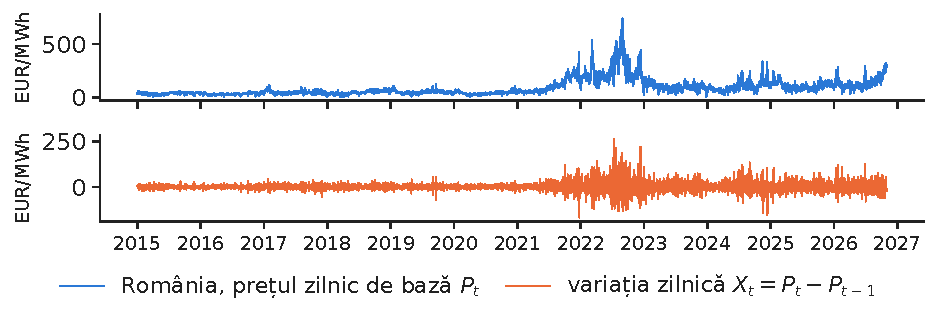
\includegraphics[width=\textwidth,height=0.433\textheight,keepaspectratio]{charts/ro/price_changes.pdf}\end{center}\vspace{-3mm}
\chartsource{Sursa: energy-charts.info (Fraunhofer ISE); prețurile PZU ale OPCOM, prin ENTSO-E; estimări proprii. Date: date zilnice, 2015-01-01 - 2026-10-31 (zile de livrare CET).}
\vspace{0.5mm}
\begin{itemize}\setlength{\itemsep}{0pt}
  \item $X_t=P_t-P_{t-1}$ = variația zilnică a prețului de bază, EUR/MWh
    \begin{itemize}\setlength{\itemsep}{0pt}
      \item Prețul poate fi negativ: folosim variații, nu randamente logaritmice
      \item Creșterea maximă: 260{,}77 (11 iulie 2022); scăderea maximă: \ensuremath{-}166{,}59 EUR/MWh (24 decembrie 2021)
    \end{itemize}
\end{itemize}
\par\vfill\manager{un furnizor care cumpără 100 MW în bandă pe PZU, la bugetul de ieri, pierde 2.400 EUR la fiecare creștere de 1 EUR/MWh.}\par\vspace{0.5mm}
\par\vfill\noindent{\scriptsize\color{FooterGray}(OPCOM; EPEX SPOT; calcule proprii)}\hfill\qlink{EMQA\_L4\_price\_changes}{Quantlets/L4/EMQA_L4_price_changes}\par\vspace{0.5mm}
\end{frame}

\begin{frame}{Valoarea la risc este o cuantilă a pierderii de mîine}
\footnotesize
\intuition{VaR este pierderea depășită doar într-o proporție mică de zile, aleasă dinainte, de exemplu o zi din o sută.}
\begin{columns}[T,onlytextwidth]
\begin{column}{0.55\textwidth}
\[ \underbrace{L_{t}=Q\cdot 24\cdot X_{t}}_{\text{pierderea, EUR}},\qquad \underbrace{\text{VaR}_{\alpha,t}=\min\{\ell:\ \Pr(L_t\le \ell\mid\mathcal F_{t-1})\ge\alpha\}}_{\text{cuantila de ordin } \alpha \text{ a pierderii}} \]{\footnotesize\begin{itemize}\setlength{\itemsep}{0pt}
  \item \textbf{\txtwhere}
    \begin{itemize}\setlength{\itemsep}{0pt}
      \item $Q$ = poziția, în MW (100 MW în bandă: $Q\cdot 24$ = 2.400 MWh pe zi)
      \item $X_t$ = variația prețului, EUR/MWh
      \item $\alpha$ = nivelul de încredere, 0{,}95 sau 0{,}99
      \item $\mathcal F_{t-1}$ = informația disponibilă pînă în ziua $t-1$ (prețurile cunoscute la ora 12:00 CET, la închiderea licitației).
    \end{itemize}
\end{itemize}\par}
\end{column}
\begin{column}{0.42\textwidth}
\begin{itemize}\setlength{\itemsep}{1pt}
  \item \textbf{Pe datele din România}, ultimele 365 de zile
    \begin{itemize}\setlength{\itemsep}{0pt}
      \item Cuantila de 99\% a lui $X_t$: 86{,}63 EUR/MWh; pentru 100 MW, VaR$_{0{,}99}$ = 207\,922 EUR
      \item Cuantila de 95\%: 50{,}39 EUR/MWh
    \end{itemize}
  \item \textbf{Ce nu spune VaR}
    \begin{itemize}\setlength{\itemsep}{0pt}
      \item Cît de mare este pierderea în cele mai proaste 1\% dintre zile
      \item Pentru aceasta avem nevoie de ES (diapozitivul următor)
    \end{itemize}
\end{itemize}
\end{column}
\end{columns}
\par\vfill\manager{biroul de tranzacționare raportează zilnic VaR de 99\%, dimineața, înainte de licitația de la ora 12:00 CET.}\par\vspace{0.5mm}
\par\vfill\noindent{\scriptsize\color{FooterGray}(Jorion, 2007; McNeil, Frey \& Embrechts, 2015)}\hfill\tryit{notebook-ul Jupyter, secțiunea 2}\par\vspace{0.5mm}
\end{frame}

\begin{frame}{Deficitul așteptat este pierderea medie dincolo de VaR}
\footnotesize
\intuition{Cînd vine o zi proastă, cît de mare este, în medie, pierderea?}
\begin{columns}[T,onlytextwidth]
\begin{column}{0.53\textwidth}
\[ \text{ES}_{\alpha,t}=\E\big[L_t\mid L_t\ge \text{VaR}_{\alpha,t}\big]=\frac{1}{1-\alpha}\int_{\alpha}^{1}\text{VaR}_{u,t}\,du \]\[ \underbrace{\text{ES}(L_1+L_2)\le\text{ES}(L_1)+\text{ES}(L_2)}_{\text{subaditivitate: diversificarea nu adaugă risc}} \]{\footnotesize\begin{itemize}\setlength{\itemsep}{0pt}
  \item \textbf{\txtwhere}
    \begin{itemize}\setlength{\itemsep}{0pt}
      \item ES este o măsură coerentă a riscului, VaR poate încălca subaditivitatea
      \item Revizuirea fundamentală a portofoliului de tranzacționare (FRTB) folosește ES de 97{,}5\% în locul VaR de 99\%.
    \end{itemize}
\end{itemize}\par}
\end{column}
\begin{column}{0.44\textwidth}
\begin{itemize}\setlength{\itemsep}{1pt}
  \item \textbf{Pe datele din România}, ultimele 365 de zile, EUR/MWh
    \begin{itemize}\setlength{\itemsep}{0pt}
      \item VaR$_{0{,}975}$ = 61{,}96; ES$_{0{,}975}$ = 86{,}91 (media celor mai proaste 10 zile)
    \end{itemize}
  \item \textbf{România + Germania--Luxemburg}, cîte 100 MW în fiecare zonă
    \begin{itemize}\setlength{\itemsep}{0pt}
      \item VaR de 99\%: 86{,}63 + 91{,}76 separat, 150{,}77 împreună
      \item Corelația 0{,}55: riscul total este mai mic
    \end{itemize}
\end{itemize}
\end{column}
\end{columns}
\par\vfill\manager{dimensionați rezerva de numerar cu ES, nu cu VaR.}\par\vspace{0.5mm}
\par\vfill\noindent{\scriptsize\color{FooterGray}(Artzner et al., 1999, Math.\ Finance; Acerbi \& Tasche, 2002, JBF; BCBS, 2019)}\hfill\tryit{notebook-ul Jupyter, secțiunea 2}\par\vspace{0.5mm}
\end{frame}

\begin{frame}{Creșterile mari de preț sînt mult mai frecvente decît prevede repartiția normală}
\small
\begin{center}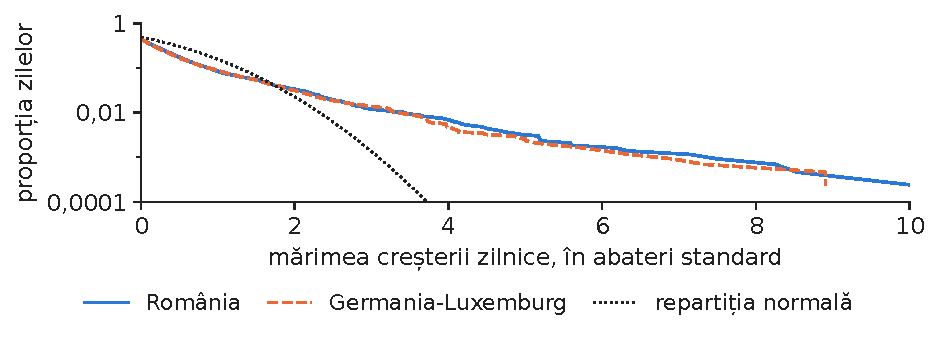
\includegraphics[width=\textwidth,height=0.430\textheight,keepaspectratio]{charts/ro/tails.pdf}\end{center}\vspace{-3mm}
\chartsource{Sursa: energy-charts.info (Fraunhofer ISE); prețurile PZU ale OPCOM (RO) și EPEX SPOT (DE-LU), prin ENTSO-E. Date: variații zilnice, 2015-01-01 - 2026-10-31.}
\vspace{0.5mm}
\begin{itemize}\setlength{\itemsep}{0pt}
  \item Excesul de aplatizare (kurtosis): 12{,}0 în România și 12{,}1 în Germania--Luxemburg (0 pentru repartiția normală)
    \begin{itemize}\setlength{\itemsep}{0pt}
      \item Creșteri de peste 3 abateri standard: 52 zile observate, față de 5{,}8 așteptate în ipoteza normalității
      \item Cea mai mare creștere are 10{,}1 abateri standard: în ipoteza normalității, ar apărea o dată la peste $10^{20}$ de ani
    \end{itemize}
\end{itemize}
\par\vfill\manager{o limită calculată cu repartiția normală subestimează frecvența zilelor de criză (cursul 1).}\par\vspace{0.5mm}
\par\vfill\noindent{\scriptsize\color{FooterGray}(calcule proprii, 1 ianuarie 2015 -- 31 octombrie 2026)}\hfill\qlink{EMQA\_L4\_tails}{Quantlets/L4/EMQA_L4_tails}\par\vspace{0.5mm}
\end{frame}

\begin{frame}{O limită calculată în 2020 cu repartiția normală a fost depășită în 2021--2022 de 19 ori mai des decît se prevedea}
\footnotesize
\intuition{O limită fixă presupune că riscul de mîine seamănă cu cel din trecut; într-o criză, această ipoteză nu se verifică.}
\begin{columns}[T,onlytextwidth]
\begin{column}{0.50\textwidth}
\[ \underbrace{\ell_{0.99}=\hat\mu+z_{0.99}\,\hat\sigma}_{\text{limita normală de 99\%}},\qquad z_{0.99}=2{,}326 \]{\footnotesize\begin{itemize}\setlength{\itemsep}{0pt}
  \item \textbf{\txtwhere}
    \begin{itemize}\setlength{\itemsep}{0pt}
      \item $\hat\mu$, $\hat\sigma$ = media și abaterea standard a lui $X_t$ în 2015--2020
      \item $z_{0{,}99}$ = cuantila de 99\% a repartiției normale standard
      \item O limită corectă este depășită în 1\% din zile.
    \end{itemize}
\end{itemize}\par}
\end{column}
\begin{column}{0.47\textwidth}
\begin{itemize}\setlength{\itemsep}{1pt}
  \item \textbf{Limita}, estimată pe 2\,182 de zile din 2015--2020
    \begin{itemize}\setlength{\itemsep}{0pt}
      \item $\hat\sigma$ = 10{,}21; limita = 23{,}77 EUR/MWh
      \item Chiar în 2015--2020: 45 depășiri, față de 21{,}8 așteptate
    \end{itemize}
  \item \textbf{Depășiri ulterioare}
    \begin{itemize}\setlength{\itemsep}{0pt}
      \item 2021--2022: 139, față de 7{,}3 așteptate
      \item 2023--2026: 226, față de 14{,}0 așteptate (de 16 ori mai multe)
    \end{itemize}
\end{itemize}
\end{column}
\end{columns}
\par\vfill\manager{o limită trebuie să urmeze volatilitatea
    \begin{itemize}\setlength{\itemsep}{0pt}
      \item Secțiunea următoare prezintă patru moduri de a o actualiza.
    \end{itemize}}\par\vspace{0.5mm}
\par\vfill\noindent{\scriptsize\color{FooterGray}(calcule proprii; cursul 1)}\hfill\tryit{notebook-ul Jupyter, secțiunea 2}\par\vspace{0.5mm}
\end{frame}


\section{Estimarea VaR și ES: patru metode}

\subsection{Simularea istorică și modelele parametrice}

\begin{frame}{Simularea istorică pe o fereastră de un an}
\footnotesize
\intuition{Ordonăm ultimele 365 de variații zilnice; a patra cea mai mare este VaR de 99\%.}
\begin{columns}[T,onlytextwidth]
\begin{column}{0.50\textwidth}
\[ \widehat{\text{VaR}}^{\text{HS}}_{\alpha,t}=\hat q_{\alpha}\big(X_{t-W},\dots,X_{t-1}\big) \]\[ \widehat{\text{ES}}^{\text{HS}}_{\alpha,t}=\text{media valorilor }\{X_s\ge\widehat{\text{VaR}}^{\text{HS}}_{\alpha,t}\} \]{\footnotesize\begin{itemize}\setlength{\itemsep}{0pt}
  \item \textbf{\txtwhere}
    \begin{itemize}\setlength{\itemsep}{0pt}
      \item $W$ = 365 de zile (fereastra)
      \item $\hat q_\alpha$ = cuantila empirică
      \item Nu se presupune nicio repartiție.
    \end{itemize}
\end{itemize}\par}
\end{column}
\begin{column}{0.47\textwidth}
\begin{itemize}\setlength{\itemsep}{1pt}
  \item \textbf{Pe datele din România}, octombrie 2026
    \begin{itemize}\setlength{\itemsep}{0pt}
      \item VaR$_{0{,}99}$ = 86{,}63; ES$_{0{,}975}$ = 87{,}59 EUR/MWh
      \item 2017--2026: depășită în 2{,}04\% din zile, nu în 1\%
    \end{itemize}
  \item \textbf{Punctul slab}
    \begin{itemize}\setlength{\itemsep}{0pt}
      \item Un regim nou are nevoie de luni de zile pentru a umple fereastra
      \item O zi de criză contează 365 de zile, apoi dispare brusc
    \end{itemize}
\end{itemize}
\end{column}
\end{columns}
\par\vfill\manager{HS este metoda implicită în multe companii energetice și reacționează cu întîrziere.}\par\vspace{0.5mm}
\par\vfill\noindent{\scriptsize\color{FooterGray}(Jorion, 2007; Christoffersen, 2012)}\hfill\tryit{notebook-ul Jupyter, secțiunea 3}\par\vspace{0.5mm}
\end{frame}

\begin{frame}{VaR parametrică: repartițiile normală și Student-$t$}
\footnotesize
\intuition{Ajustăm o curbă pe variațiile din ultimul an și citim cuantila ei; curba Student-$t$ are cozi mai groase.}
\begin{columns}[T,onlytextwidth]
\begin{column}{0.55\textwidth}
\[ \text{VaR}^{N}_{\alpha}=\mu+\sigma z_\alpha,\qquad \text{ES}^{N}_{\alpha}=\mu+\sigma\frac{\varphi(z_\alpha)}{1-\alpha} \]\[ \text{VaR}^{t}_{\alpha}=m+s\,t_{\nu,\alpha},\qquad \text{ES}^{t}_{\alpha}=m+s\,\frac{g_\nu(t_{\nu,\alpha})}{1-\alpha}\cdot\frac{\nu+t_{\nu,\alpha}^2}{\nu-1} \]{\footnotesize\begin{itemize}\setlength{\itemsep}{0pt}
  \item \textbf{\txtwhere}
    \begin{itemize}\setlength{\itemsep}{0pt}
      \item $\mu,\sigma$ = media, abaterea standard
      \item $z_\alpha$, $\varphi$ = cuantila și densitatea normală standard
      \item $m,s,\nu$ = locația, scala, gradele de libertate, estimate prin metoda verosimilității maxime (MLE)
      \item $t_{\nu,\alpha}$, $g_\nu$ = cuantila și densitatea Student-$t$ (Anexa A).
    \end{itemize}
\end{itemize}\par}
\end{column}
\begin{column}{0.42\textwidth}
\begin{itemize}\setlength{\itemsep}{1pt}
  \item \textbf{Pe datele din România}, octombrie 2026, EUR/MWh
    \begin{itemize}\setlength{\itemsep}{0pt}
      \item Normală: VaR$_{0{,}99}$ = 69{,}64; ES$_{0{,}975}$ = 69{,}98
      \item Student-$t$: VaR$_{0{,}99}$ = 76{,}66; ES$_{0{,}975}$ = 80{,}05
    \end{itemize}
  \item \textbf{Testarea retrospectivă}, zile peste VaR de 99\%
    \begin{itemize}\setlength{\itemsep}{0pt}
      \item Normală: 3{,}21\%; Student-$t$: 1{,}98\% (ținta: 1\%)
      \item La 95\%, curba $t$ este prea îngustă: 8{,}75\%
    \end{itemize}
\end{itemize}
\end{column}
\end{columns}
\par\vfill\manager{VaR normală este cel mai ușor de explicat și cel mai periculos de folosit fără verificare.}\par\vspace{0.5mm}
\par\vfill\noindent{\scriptsize\color{FooterGray}(McNeil, Frey \& Embrechts, 2015)}\hfill\tryit{notebook-ul Jupyter, secțiunea 3}\par\vspace{0.5mm}
\end{frame}

\subsection{Simularea istorică filtrată și valorile extreme}

\begin{frame}{Simularea istorică filtrată: șocurile trecute, rescalate la volatilitatea curentă}
\footnotesize
\intuition{Împărțim variațiile trecute la volatilitatea lor, apoi înmulțim șocurile cu volatilitatea de azi.}
\begin{columns}[T,onlytextwidth]
\begin{column}{0.53\textwidth}
\[ e_t=X_t-\mu_{d(t)},\quad \sigma_t^2=\omega+a\,e_{t-1}^2+b\,\sigma_{t-1}^2,\quad z_t=e_t/\sigma_t \]\[ \text{VaR}^{\text{FHS}}_{\alpha,t}=\mu_{d(t)}+\sigma_t\,\hat q_\alpha(z) \]{\footnotesize\begin{itemize}\setlength{\itemsep}{0pt}
  \item \textbf{\txtwhere}
    \begin{itemize}\setlength{\itemsep}{0pt}
      \item $\mu_{d(t)}$ = variația medie a zilei din săptămînă (prețul scade la sfîrșit de săptămînă)
      \item $\sigma_t$ = volatilitatea din modelul autoregresiv generalizat cu heteroscedasticitate condiționată (GARCH), cursul 3, reestimat la 21 de zile pe 730 de zile
      \item ES: $\sigma_t$ înmulțit cu media valorilor $z$ peste $\hat q_\alpha(z)$.
    \end{itemize}
\end{itemize}\par}
\end{column}
\begin{column}{0.44\textwidth}
\begin{itemize}\setlength{\itemsep}{1pt}
  \item \textbf{Pe datele din România}, GARCH(1,1)
    \begin{itemize}\setlength{\itemsep}{0pt}
      \item $\sigma_t$ între 4{,}06 (29 martie 2021) și 100{,}86 EUR/MWh (12 iulie 2022)
      \item Octombrie 2026: VaR$_{0{,}99}$ = 67{,}50 EUR/MWh
    \end{itemize}
  \item \textbf{Testarea retrospectivă}
    \begin{itemize}\setlength{\itemsep}{0pt}
      \item 99\%: 1{,}51\% din zile
      \item 95\%: 5{,}58\%; Kupiec: $p$ = 0{,}120
    \end{itemize}
\end{itemize}
\end{column}
\end{columns}
\par\vfill\manager{FHS ridică limita la cîteva zile după un salt al volatilității
    \begin{itemize}\setlength{\itemsep}{0pt}
      \item HS are nevoie de luni.
    \end{itemize}}\par\vspace{0.5mm}
\par\vfill\noindent{\scriptsize\color{FooterGray}(Barone-Adesi, Giannopoulos \& Vosper, 1999; Bollerslev, 1986)}\hfill\tryit{notebook-ul Jupyter, secțiunea 3}\par\vspace{0.5mm}
\end{frame}

\begin{frame}{Teoria valorilor extreme: modelăm numai coada, cu o curbă Pareto generalizată}
\footnotesize
\intuition{Peste un prag ridicat, excesele aproape oricărei repartiții urmează aceeași curbă cu doi parametri.}
\begin{columns}[T,onlytextwidth]
\begin{column}{0.55\textwidth}
\[ \Pr(Z-u\le y\mid Z>u)\approx 1-\Big(1+\frac{\xi y}{\beta}\Big)^{-1/\xi} \]\[ \text{VaR}_\alpha=u+\frac{\beta}{\xi}\Big[\Big(\frac{n}{N_u}(1-\alpha)\Big)^{-\xi}-1\Big],\quad \text{ES}_\alpha=\frac{\text{VaR}_\alpha+\beta-\xi u}{1-\xi} \]{\footnotesize\begin{itemize}\setlength{\itemsep}{0pt}
  \item \textbf{\txtwhere}
    \begin{itemize}\setlength{\itemsep}{0pt}
      \item Metoda depășirilor unui prag (POT): $u$ = cuantila de 90\% a lui $z$, depășită de $N_u$ din cele $n$ reziduuri
      \item Repartiția Pareto generalizată (GPD): forma $\xi$ (grosimea cozii), scala $\beta$, estimate prin MLE
      \item Apoi înmulțim cu $\sigma_t$, ca la FHS (Anexa B).
    \end{itemize}
\end{itemize}\par}
\end{column}
\begin{column}{0.42\textwidth}
\begin{itemize}\setlength{\itemsep}{1pt}
  \item \textbf{Variațiile brute}, pragul = cuantila de 95\%
    \begin{itemize}\setlength{\itemsep}{0pt}
      \item $\hat\xi$ = 0{,}164: o coadă groasă
      \item Momentele de ordin peste 6{,}1 nu există
    \end{itemize}
  \item \textbf{După filtrul GARCH}
    \begin{itemize}\setlength{\itemsep}{0pt}
      \item $\hat\xi$ median = 0{,}011: filtrul preia cea mai mare parte a cozii
      \item Testarea VaR de 99\%: 1{,}37\% din zile, cel mai bun rezultat
    \end{itemize}
\end{itemize}
\end{column}
\end{columns}
\par\vfill\manager{folosiți EVT pentru ziua care apare o dată la zece ani și nu se află în nicio fereastră.}\par\vspace{0.5mm}
\par\vfill\noindent{\scriptsize\color{FooterGray}(Pickands, 1975; McNeil \& Frey, 2000; Chan \& Gray, 2006, IJF)}\hfill\tryit{notebook-ul Jupyter, secțiunea 3}\par\vspace{0.5mm}
\end{frame}

\begin{frame}{Peste prag, curba Pareto urmează datele, iar curba normală nu}
\small
\begin{center}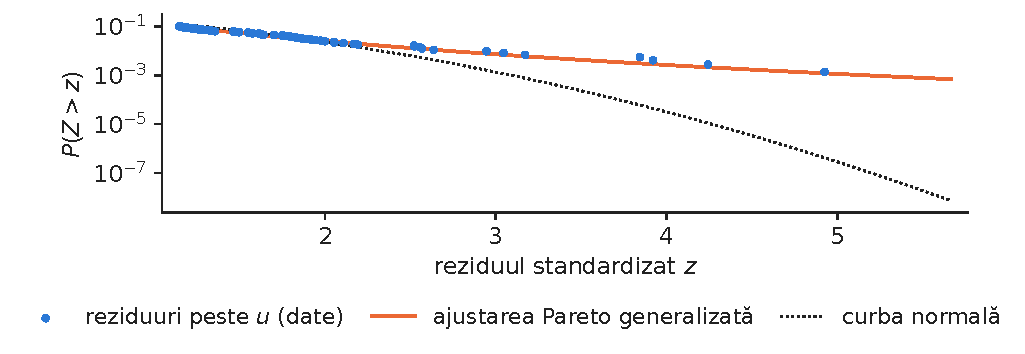
\includegraphics[width=\textwidth,height=0.455\textheight,keepaspectratio]{charts/ro/gpd_tail.pdf}\end{center}\vspace{-3mm}
\chartsource{Sursa: energy-charts.info (Fraunhofer ISE); prețurile PZU ale OPCOM, prin ENTSO-E; estimări proprii. Date: variații filtrate GARCH, cele 730 de zile dinainte de 2026-10-31.}
\vspace{0.5mm}
\begin{itemize}\setlength{\itemsep}{0pt}
  \item Ultima reestimare (11 octombrie 2026): $\hat\xi$ = 0{,}182, $\hat\beta$ = 0{,}569
    \begin{itemize}\setlength{\itemsep}{0pt}
      \item $\hat\xi>0$ în 53\% din reestimări: coada reziduurilor standardizate este uneori groasă, alteori nu
    \end{itemize}
\end{itemize}
\par\vfill\manager{o zi de 4 abateri standard este rară, dar posibilă
    \begin{itemize}\setlength{\itemsep}{0pt}
      \item Curba normală o consideră practic imposibilă.
    \end{itemize}}\par\vspace{0.5mm}
\par\vfill\noindent{\scriptsize\color{FooterGray}(Balkema \& de Haan, 1974; McNeil \& Frey, 2000)}\hfill\qlink{EMQA\_L4\_gpd\_tail}{Quantlets/L4/EMQA_L4_gpd_tail}\par\vspace{0.5mm}
\end{frame}

\subsection{Compararea metodelor}

\begin{frame}{VaR și ES pentru aceeași zi, estimate prin cinci metode}
\footnotesize
\begin{center}{\footnotesize\renewcommand{\arraystretch}{1.2}\setlength{\tabcolsep}{4pt}
\begin{tabular}{@{}lrrrrr@{}}\toprule
Metoda & VaR$_{0{,}95}$ & VaR$_{0{,}99}$ & ES$_{0{,}975}$ & VaR$_{0{,}99}$, mii EUR & ES$_{0{,}975}$, mii EUR \\ \midrule
HS & 50{,}38 & 86{,}63 & 87{,}59 & 208 & 210 \\
Normală & 49{,}33 & 69{,}64 & 69{,}98 & 167 & 168 \\
Student-$t$ & 45{,}77 & 76{,}66 & 80{,}05 & 184 & 192 \\
FHS & 36{,}22 & 67{,}50 & 67{,}44 & 162 & 162 \\
EVT & 35{,}66 & 64{,}33 & 68{,}54 & 154 & 164 \\
\bottomrule\end{tabular}}\end{center}\vspace{-1mm}
\par\vspace{0.5mm}{\scriptsize \begin{itemize}\setlength{\itemsep}{0pt}
  \item Media celor 31 prognoze pentru zilele din octombrie 2026; primele trei coloane în EUR/MWh; ultimele două pentru 100 MW în bandă (2.400 MWh pe zi).
\end{itemize}}\begin{itemize}\setlength{\itemsep}{1pt}
  \item \textbf{Cum citim tabelul}
    \begin{itemize}\setlength{\itemsep}{0pt}
      \item HS și Student-$t$ conțin încă zilele volatile din ultimul an
      \item FHS și EVT folosesc volatilitatea actuală, sub media anului în octombrie 2026
    \end{itemize}
\end{itemize}
\par\vfill\manager{raportați două metode alăturate și explicați diferența dintre ele.}\par\vspace{0.5mm}
\par\vfill\noindent{\scriptsize\color{FooterGray}(estimări proprii)}\hfill\tryit{notebook-ul Jupyter, secțiunea 3}\par\vspace{0.5mm}
\end{frame}

\begin{frame}{În criză, FHS s-a adaptat repede, iar HS și VaR normală au întîrziat}
\small
\begin{center}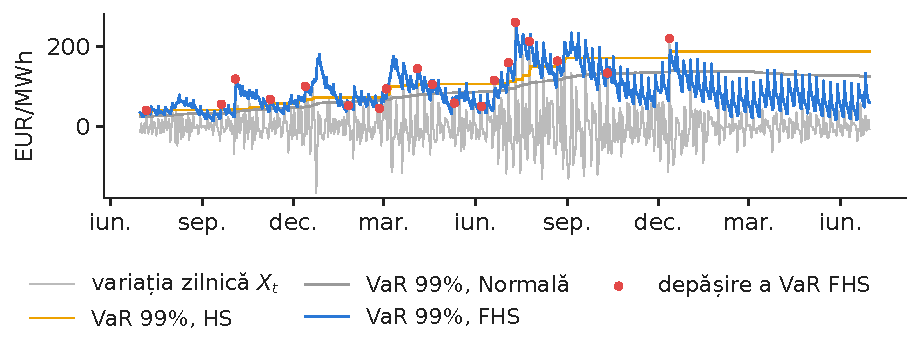
\includegraphics[width=\textwidth,height=0.521\textheight,keepaspectratio]{charts/ro/var_paths.pdf}\end{center}\vspace{-3mm}
\chartsource{Sursa: energy-charts.info (Fraunhofer ISE); prețurile PZU ale OPCOM, prin ENTSO-E; estimări proprii. Date: prognoze pentru 2021-07-01 - 2023-06-30.}
\vspace{0.5mm}
\begin{itemize}\setlength{\itemsep}{0pt}
  \item Depășiri ale VaR de 99\%, 1 iulie 2021 -- 30 iunie 2023 (730 de zile, 7{,}3 depășiri așteptate)
    \begin{itemize}\setlength{\itemsep}{0pt}
      \item HS: 28; normală: 45; Student-$t$: 29; FHS: 19; EVT: 17
    \end{itemize}
\end{itemize}
\par\vfill\manager{într-o criză, un model care reacționează în cîteva zile protejează lichiditățile.}\par\vspace{0.5mm}
\par\vfill\noindent{\scriptsize\color{FooterGray}(estimări proprii)}\hfill\qlink{EMQA\_L4\_var\_paths}{Quantlets/L4/EMQA_L4_var_paths}\par\vspace{0.5mm}
\end{frame}

\begin{frame}{Regula rădăcinii pătrate a timpului supraestimează riscul pe 10 zile}
\small
\begin{center}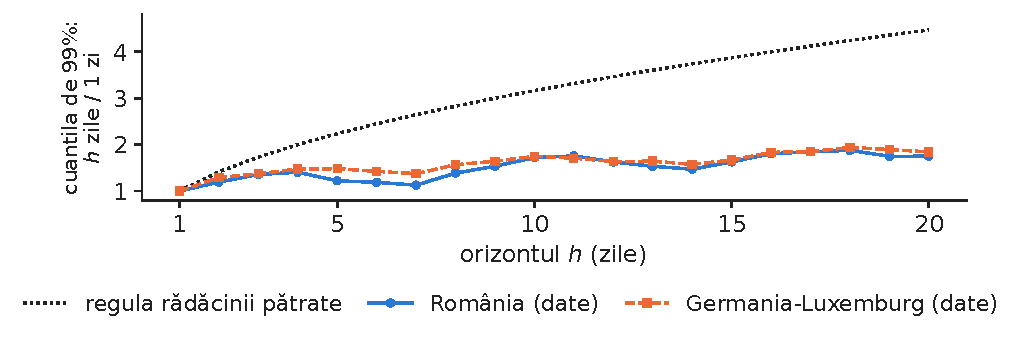
\includegraphics[width=\textwidth,height=0.415\textheight,keepaspectratio]{charts/ro/horizon.pdf}\end{center}\vspace{-3mm}
\chartsource{Sursa: energy-charts.info (Fraunhofer ISE); prețurile PZU ale OPCOM (RO) și EPEX SPOT (DE-LU), prin ENTSO-E. Date: prețuri zilnice de bază, 2015-01-01 - 2026-10-31.}
\vspace{0.5mm}
\begin{itemize}\setlength{\itemsep}{0pt}
  \item Cuantila de 99\% pe 10 zile = 1{,}72 $\times$ cea pe o zi (RO; 1{,}75 în DE-LU), nu $\sqrt{10}$ = 3{,}16
    \begin{itemize}\setlength{\itemsep}{0pt}
      \item Raportul varianțelor la 10 zile: 0{,}33 (1 = mers aleator); autocorelația lui $X_t$: \ensuremath{-}0{,}076 (decalaj 1), 0{,}474 (decalaj 7)
    \end{itemize}
\end{itemize}
\par\vfill\manager{măsurați direct variațiile pe 10 zile
    \begin{itemize}\setlength{\itemsep}{0pt}
      \item Înmulțirea cu $\sqrt{10}$ blochează capital inutil.
    \end{itemize}}\par\vspace{0.5mm}
\par\vfill\noindent{\scriptsize\color{FooterGray}(calcule proprii; Weron, 2014, IJF)}\hfill\qlink{EMQA\_L4\_horizon}{Quantlets/L4/EMQA_L4_horizon}\par\vspace{0.5mm}
\end{frame}


\section{Testarea retrospectivă a VaR și ES}

\begin{frame}{Testul Kupiec pentru frecvența depășirilor}
\footnotesize
\intuition{O VaR de 99\% promite că va fi depășită în 1\% din zile; numărăm depășirile și testăm dacă proporția lor diferă de 1\%.}
\begin{columns}[T,onlytextwidth]
\begin{column}{0.52\textwidth}
\[ I_t=\mathbf 1\{L_t>\text{VaR}_{\alpha,t}\},\qquad x=\textstyle\sum_{t=1}^{n}I_t,\qquad \hat p=x/n \]\[ \text{LR}_{uc}=-2\ln\frac{(1-p)^{n-x}\,p^{x}}{(1-\hat p)^{n-x}\,\hat p^{\,x}}\ \sim\ \chi^2_1 \]{\footnotesize\begin{itemize}\setlength{\itemsep}{0pt}
  \item \textbf{\txtwhere}
    \begin{itemize}\setlength{\itemsep}{0pt}
      \item $I_t$ = indicatorul depășirii
      \item $p=1-\alpha$ = proporția promisă
      \item Testul raportului de verosimilitate (LR) pentru acoperirea necondiționată
      \item Respingem la pragul de 5\% dacă LR$_{uc}>$ 3{,}84.
    \end{itemize}
\end{itemize}\par}
\end{column}
\begin{column}{0.45\textwidth}
\begin{itemize}\setlength{\itemsep}{1pt}
  \item \textbf{Pe datele din România}, VaR de 99\%, 3\,587 de zile
    \begin{itemize}\setlength{\itemsep}{0pt}
      \item Depășiri așteptate: 35{,}9
      \item Normală: 115, LR$_{uc}$ = 111{,}5; FHS: 54, LR$_{uc}$ = 8{,}0
      \item EVT: 49, $p$ = 0{,}037
    \end{itemize}
  \item \textbf{Puterea testului}
    \begin{itemize}\setlength{\itemsep}{0pt}
      \item Pe un singur an, la 99\%, ne așteptăm la doar 2--3 depășiri; testul respinge foarte greu
      \item Zece ani de date zilnice îl fac precis
    \end{itemize}
\end{itemize}
\end{column}
\end{columns}
\par\vfill\manager{cereți numărul depășirilor înainte de a avea încredere în VaR raportată de cineva.}\par\vspace{0.5mm}
\par\vfill\noindent{\scriptsize\color{FooterGray}(Kupiec, 1995, J.\ Derivatives)}\hfill\tryit{notebook-ul Jupyter, secțiunea 4}\par\vspace{0.5mm}
\end{frame}

\begin{frame}{Testul Christoffersen pentru independența depășirilor}
\footnotesize
\intuition{Un model bun nu este surprins de două ori la rînd: o depășire azi nu trebuie să facă mai probabilă o depășire mîine.}
\begin{columns}[T,onlytextwidth]
\begin{column}{0.55\textwidth}
\[ \pi_{01}=\Pr(I_t=1\mid I_{t-1}=0),\qquad \pi_{11}=\Pr(I_t=1\mid I_{t-1}=1) \]\[ \text{LR}_{ind}=-2\ln\frac{(1-\hat\pi)^{n_{00}+n_{10}}\hat\pi^{\,n_{01}+n_{11}}}{(1-\hat\pi_{01})^{n_{00}}\hat\pi_{01}^{\,n_{01}}(1-\hat\pi_{11})^{n_{10}}\hat\pi_{11}^{\,n_{11}}}\sim\chi^2_1 \]{\footnotesize\begin{itemize}\setlength{\itemsep}{0pt}
  \item \textbf{\txtwhere}
    \begin{itemize}\setlength{\itemsep}{0pt}
      \item $n_{ij}$ = numărul zilelor cu $I_{t-1}=i$ și $I_t=j$
      \item $\hat\pi$ = proporția totală
      \item $H_0$: $\pi_{01}=\pi_{11}$
      \item Testul comun LR$_{cc}$ = LR$_{uc}$ + LR$_{ind}\sim\chi^2_2$.
    \end{itemize}
\end{itemize}\par}
\end{column}
\begin{column}{0.42\textwidth}
\begin{itemize}\setlength{\itemsep}{1pt}
  \item \textbf{Pe datele din România}, VaR de 99\%, valorile $p$ ale testului de independență
    \begin{itemize}\setlength{\itemsep}{0pt}
      \item HS: 0{,}682; normală: 0{,}868; FHS: 0{,}199
      \item Nicio metodă nu îl pică: depășirile cad rareori în zile consecutive
    \end{itemize}
  \item \textbf{Dar se grupează pe luni}
    \begin{itemize}\setlength{\itemsep}{0pt}
      \item Normală: 7{,}26\% din zile în 2021--2022, 2{,}33\% în 2017--2020
      \item Un test de ordinul întîi nu observă acest lucru; semaforul Basel îl observă
    \end{itemize}
\end{itemize}
\end{column}
\end{columns}
\par\vfill\manager{urmăriți momentul în care apar depășirile, nu doar numărul lor.}\par\vspace{0.5mm}
\par\vfill\noindent{\scriptsize\color{FooterGray}(Christoffersen, 1998, IER)}\hfill\tryit{notebook-ul Jupyter, secțiunea 4}\par\vspace{0.5mm}
\end{frame}

\begin{frame}{În zece ani, doar metodele filtrate trec testul la 95\%; la 99\%, toate metodele au prea multe depășiri}
\footnotesize
\begin{center}{\footnotesize\renewcommand{\arraystretch}{1.2}\setlength{\tabcolsep}{4pt}
\begin{tabular}{@{}lrrrrrrr@{}}\toprule
România & 95\%: proporția & Kupiec $p$ & 99\%: număr & proporția, \% & Kupiec $p$ & Christoffersen $p$ & zile roșii, \% \\ \midrule
HS & \cellcolor{Forest!23}6{,}16 & 0{,}002 & 73 & \cellcolor{Forest!3}2{,}04 & $<$0{,}001 & 0{,}682 & \cellcolor{Crimson!6}16{,}7 \\
Normală & \cellcolor{Crimson!10}7{,}36 & $<$0{,}001 & 115 & \cellcolor{Crimson!55}3{,}21 & $<$0{,}001 & 0{,}868 & \cellcolor{Crimson!53}29{,}5 \\
Student-$t$ & \cellcolor{Crimson!48}8{,}75 & $<$0{,}001 & 71 & \cellcolor{Forest!6}1{,}98 & $<$0{,}001 & 0{,}630 & \cellcolor{Crimson!12}18{,}3 \\
FHS & \cellcolor{Forest!39}5{,}58 & 0{,}120 & 54 & \cellcolor{Forest!30}1{,}51 & 0{,}005 & 0{,}199 & \cellcolor{Forest!32}6{,}2 \\
EVT & \cellcolor{Forest!40}5{,}55 & 0{,}139 & 49 & \cellcolor{Forest!36}1{,}37 & 0{,}037 & 0{,}244 & \cellcolor{Forest!45}2{,}8 \\
\bottomrule\end{tabular}}\end{center}\vspace{-1mm}
\par\vspace{0.5mm}{\scriptsize \begin{itemize}\setlength{\itemsep}{0pt}
  \item Testare retrospectivă 1 ianuarie 2017 -- 31 octombrie 2026; așteptat: 5\% și 1\% din 3\,587 de zile (35{,}9 la 99\%); verde = aproape de țintă, roșu = departe.
  \item Zile roșii = proporția zilelor în care ultimele 250 de zile conțin cel puțin 10 depășiri (diapozitivul următor); Germania--Luxemburg: Anexa D.
\end{itemize}}
\par\vfill\manager{acceptați un model la 95\%, dar păstrați capital suplimentar pentru coada de 99\%, pe care niciun model nu o surprinde complet.}\par\vspace{0.5mm}
\par\vfill\noindent{\scriptsize\color{FooterGray}(Kupiec, 1995; Christoffersen, 1998; estimări proprii)}\hfill\tryit{notebook-ul Jupyter, secțiunea 4}\par\vspace{0.5mm}
\end{frame}

\begin{frame}{Semaforul Basel: VaR normală a stat 30\% din zile în zona roșie}
\small
\begin{center}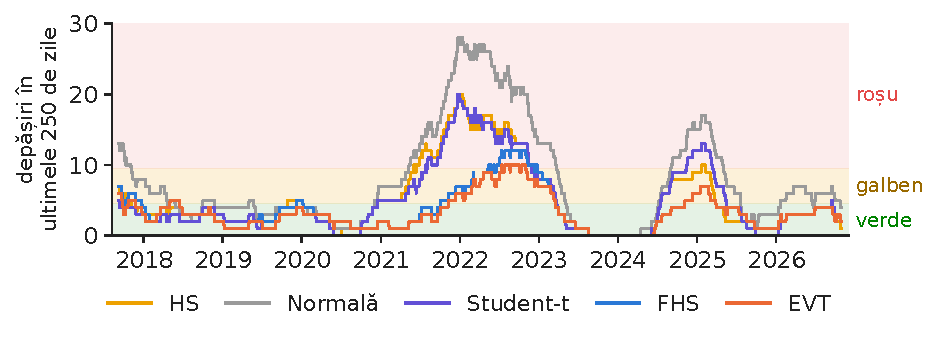
\includegraphics[width=\textwidth,height=0.430\textheight,keepaspectratio]{charts/ro/traffic.pdf}\end{center}\vspace{-3mm}
\chartsource{Sursa: energy-charts.info (Fraunhofer ISE); prețurile PZU ale OPCOM, prin ENTSO-E; estimări proprii. Date: testare retrospectivă 2017-01-01 - 2026-10-31, VaR 99\%.}
\vspace{0.5mm}
\begin{itemize}\setlength{\itemsep}{0pt}
  \item Numărul depășirilor VaR de 99\% în ultimele 250 de zile: verde 0--4, galben 5--9, roșu 10 sau mai multe după Comitetul de la Basel pentru Supraveghere Bancară (BCBS)
    \begin{itemize}\setlength{\itemsep}{0pt}
      \item Un model corect este în zona verde cu probabilitatea 89{,}2\% și în zona roșie cu 0{,}025\%
      \item Zile în zona roșie: HS 16{,}7\%, FHS 6{,}2\%, EVT 2{,}8\%
    \end{itemize}
\end{itemize}
\par\vfill\manager{zona galbenă cere recalibrarea modelului, iar cea roșie oprirea lui pentru limite.}\par\vspace{0.5mm}
\par\vfill\noindent{\scriptsize\color{FooterGray}(BCBS, 1996)}\hfill\qlink{EMQA\_L4\_traffic}{Quantlets/L4/EMQA_L4_traffic}\par\vspace{0.5mm}
\end{frame}

\begin{frame}{În 2021--2022 toate metodele au eșuat; din 2023, metodele filtrate au revenit aproape de 1\%}
\footnotesize
\begin{center}{\footnotesize\renewcommand{\arraystretch}{1.2}\setlength{\tabcolsep}{4pt}
\begin{tabular}{@{}lrrrrrr@{}}\toprule
VaR 99\%, \% din zile & RO 17--20 & RO 21--22 & RO 23--26 & DE-LU 17--20 & DE-LU 21--22 & DE-LU 23--26 \\ \midrule
HS & \cellcolor{Forest!39}1{,}58 & \cellcolor{Crimson!53}4{,}93 & \cellcolor{Forest!55}1{,}00 & \cellcolor{Forest!51}1{,}16 & \cellcolor{Crimson!23}3{,}84 & \cellcolor{Forest!53}1{,}07 \\
Normală & \cellcolor{Forest!18}2{,}33 & \cellcolor{Crimson!55}7{,}26 & \cellcolor{Forest!28}2{,}00 & \cellcolor{Forest!17}2{,}40 & \cellcolor{Crimson!55}5{,}89 & \cellcolor{Forest!26}2{,}07 \\
Student-$t$ & \cellcolor{Forest!47}1{,}30 & \cellcolor{Crimson!46}4{,}66 & \cellcolor{Forest!47}1{,}29 & \cellcolor{Forest!45}1{,}37 & \cellcolor{Crimson!27}3{,}97 & \cellcolor{Forest!47}1{,}29 \\
FHS & \cellcolor{Forest!45}1{,}37 & \cellcolor{Forest!3}2{,}88 & \cellcolor{Forest!53}0{,}93 & \cellcolor{Forest!43}1{,}44 & \cellcolor{Forest!15}2{,}47 & \cellcolor{Forest!45}1{,}36 \\
EVT & \cellcolor{Forest!48}1{,}24 & \cellcolor{Forest!15}2{,}47 & \cellcolor{Forest!53}0{,}93 & \cellcolor{Forest!41}1{,}51 & \cellcolor{Forest!22}2{,}19 & \cellcolor{Forest!53}1{,}07 \\
\bottomrule\end{tabular}}\end{center}\vspace{-1mm}\begin{itemize}\setlength{\itemsep}{1pt}
  \item \textbf{Criza}
    \begin{itemize}\setlength{\itemsep}{0pt}
      \item Chiar și FHS a fost depășită în 2{,}88\% din zile în România: șocul gazelor a mutat întreaga repartiție
    \end{itemize}
  \item \textbf{După criză}
    \begin{itemize}\setlength{\itemsep}{0pt}
      \item FHS: 0{,}93\%; EVT: 0{,}93\%; HS: 1{,}00\%; normală: 2{,}00\%
    \end{itemize}
\end{itemize}
\par\vfill\manager{testați orice model pe 2021--2022 înainte de a vă baza pe el într-o criză.}\par\vspace{0.5mm}
\par\vfill\noindent{\scriptsize\color{FooterGray}(estimări proprii)}\hfill\tryit{notebook-ul Jupyter, secțiunea 4}\par\vspace{0.5mm}
\end{frame}

\begin{frame}{Testarea ES: mărimea pierderilor de dincolo de VaR}
\footnotesize
\intuition{Împărțim fiecare pierdere din zilele cu depășiri la prognoza ES; dacă ES este corect, media este 1.}
\begin{columns}[T,onlytextwidth]
\begin{column}{0.45\textwidth}
\[ Z_2=\frac{1}{T(1-\alpha)}\sum_{t=1}^{T}\frac{L_t\,I_t}{\text{ES}_{\alpha,t}}-1,\qquad \E_{H_0}[Z_2]=0 \]{\footnotesize\begin{itemize}\setlength{\itemsep}{0pt}
  \item \textbf{\txtwhere}
    \begin{itemize}\setlength{\itemsep}{0pt}
      \item $\alpha$ = 0{,}975
      \item $I_t$ = depășirea VaR$_{0{,}975}$
      \item $Z_2>0$ = ES prea mic
      \item Valoarea $p$: 2.000 de traiectorii simulate din fiecare model (Anexa C).
    \end{itemize}
\end{itemize}\par}
\end{column}
\begin{column}{0.52\textwidth}
{\scriptsize\renewcommand{\arraystretch}{1.1}\setlength{\tabcolsep}{4pt}
\begin{tabular}{@{}lrrrrrr@{}}\toprule
$Z_2$ & total & $p$ & 2021--22 & $p$ & 2023--26 & $p$ \\ \midrule
HS & 0{,}628 & $<$0{,}001 & 2{,}694 & $<$0{,}001 & \ensuremath{-}0{,}026 & 0{,}761 \\
Normală & 1{,}425 & $<$0{,}001 & 4{,}170 & $<$0{,}001 & 0{,}697 & $<$0{,}001 \\
Student-$t$ & 0{,}908 & $<$0{,}001 & 2{,}910 & $<$0{,}001 & 0{,}329 & 0{,}052 \\
FHS & 0{,}335 & 0{,}004 & 1{,}164 & $<$0{,}001 & \ensuremath{-}0{,}083 & 0{,}759 \\
EVT & 0{,}279 & 0{,}009 & 1{,}183 & $<$0{,}001 & \ensuremath{-}0{,}114 & 0{,}722 \\
\bottomrule\end{tabular}}\par\vspace{1mm}\begin{itemize}\setlength{\itemsep}{1pt}
  \item \textbf{Interpretare}: în criză, toate prognozele ES au fost prea mici
    \begin{itemize}\setlength{\itemsep}{0pt}
      \item Din 2023, FHS, EVT și HS trec testul.
    \end{itemize}
\end{itemize}
\end{column}
\end{columns}
\par\vfill\manager{evaluați ES pe mai mulți ani, niciodată pe un trimestru (circa 9 zile extreme pe an).}\par\vspace{0.5mm}
\par\vfill\noindent{\scriptsize\color{FooterGray}(Acerbi \& Székely, 2014; Pele \& Mazurencu-Marinescu-Pele, 2026)}\hfill\tryit{notebook-ul Jupyter, secțiunea 4}\par\vspace{0.5mm}
\end{frame}

\begin{frame}{AIDA 2026: deplasarea conformală corectează erorile de calibrare ale VaR}
\footnotesize
\begin{itemize}\setlength{\itemsep}{1pt}
  \item \textbf{Ce a făcut lucrarea} (D.\,T.\ Pele, conferința AIDA (AI and Digital Assets in Energy and Finance), 4 iunie 2026)
    \begin{itemize}\setlength{\itemsep}{0pt}
      \item Scorul $s_t=\hat q_t-r_t$ ($>0$ în ziua unei depășiri); $\hat q_V$ = cuantila de 99\% a scorurilor trecute; VaR corectată = VaR + $\hat q_V$, fixă (audit) sau glisantă pe 250 de zile
      \item VaR de 1\% a 10 modele (fundaționale, de tip GARCH, HS) pe 24 de active, inclusiv petrol și gaze: 240 de perechi; Kupiec, Christoffersen, semaforul Basel
    \end{itemize}
  \item \textbf{Ce a găsit}
    \begin{itemize}\setlength{\itemsep}{0pt}
      \item $\hat q_V$ între $-$0{,}007 (prea prudent) și +0{,}102 (fără informație despre coadă); explică 53{,}4\% ($R^2$ parțial) din cîștigul la scorul cuantilic
      \item Perechi în zona verde: 63/240 (26{,}2\%) inițial, 203/240 (84{,}6\%) fix, 234/240 (97{,}5\%) glisant
      \item Rata depășirilor este refăcută, gruparea lor nu
    \end{itemize}
  \item \textbf{Legătura cu acest curs}
    \begin{itemize}\setlength{\itemsep}{0pt}
      \item Testul Kupiec arată dacă VaR eșuează, $\hat q_V$ cu cît; lărgirea garanției $\hat c_t$ (secțiunea 4) este aceeași deplasare
    \end{itemize}
\end{itemize}
\par\vspace{0.5mm}{\scriptsize \begin{itemize}\setlength{\itemsep}{0pt}
  \item Rezultatele sînt cele raportate de autori; prezentarea: \href{https://github.com/danpele/EMQA/blob/main/resources/aida2026/pele_conformal_tail_risk.pdf}{diapozitive}; lucrare trimisă spre publicare.
\end{itemize}}
\par\vfill\manager{după un test eșuat, lărgiți VaR cu deplasarea conformală și testați în continuare gruparea depășirilor.}\par\vspace{0.5mm}
\par\vfill\noindent{\scriptsize\color{FooterGray}(Pele, Bolovăneanu, Ginavar, Lessmann \& Härdle, AIDA, ASE, 4 iunie 2026)}\par\vspace{0.5mm}
\end{frame}


\section{De la cuantile la marje, garanții și limite}

\subsection{Marjele la bursă}

\begin{frame}{Marjele la bursă: marja inițială ca VaR, marja de variație plătită zilnic}
\footnotesize
\intuition{Casa de compensare reține un depozit pentru pierderea de 99\% pe două zile și decontează zilnic diferențele.}
\begin{columns}[T,onlytextwidth]
\begin{column}{0.45\textwidth}
\[ \underbrace{\text{IM}_t=K F_t\,\hat q_{0{,}99}\big(|r^{(2)}|\big)}_{\text{marja inițială}},\quad \underbrace{\text{VM}_t=n K(F_t-F_{t-1})}_{\text{marja de variație}} \]{\footnotesize\begin{itemize}\setlength{\itemsep}{0pt}
  \item \textbf{\txtwhere}
    \begin{itemize}\setlength{\itemsep}{0pt}
      \item Marja inițială (IM) și de variație (VM), cerute de contrapartea centrală (CCP)
      \item $F_t$ = prețul futures, $K$ = 1.000 de barili (un lot Brent)
      \item $r^{(2)}$ = randamentul pe două zile
      \item $n$ = loturi vîndute (+) sau cumpărate ($-$).
    \end{itemize}
\end{itemize}\par}
\end{column}
\begin{column}{0.52\textwidth}
\begin{itemize}\setlength{\itemsep}{1pt}
  \item \textbf{Regulamentul privind infrastructura pieței europene (EMIR)}, standardele tehnice de reglementare (RTS) 153/2013
    \begin{itemize}\setlength{\itemsep}{0pt}
      \item Futures: 99\%, lichidare în 2 zile, minimum 12 luni de date (art.~24--26)
      \item Instrumente anticiclice (APC), art.~28: o rezervă de 25\%, o pondere de 25\% pentru zilele de criză sau un prag pe 10 ani
    \end{itemize}
  \item \textbf{Brent, Intercontinental Exchange (ICE)}, 100 de loturi vîndute: VM maximă într-o zi 0{,}88 mil.\ USD (16 septembrie 2019)
\end{itemize}
\end{column}
\end{columns}
\par\vfill\manager{producătorul acoperit cîștigă mai tîrziu din vînzarea fizică, dar plătește marja azi.}\par\vspace{0.5mm}
\par\vfill\noindent{\scriptsize\color{FooterGray}(Regulamentul delegat (UE) 153/2013; ICE Futures Europe)}\hfill\tryit{notebook-ul Jupyter, secțiunea 5}\par\vspace{0.5mm}
\end{frame}

\begin{frame}{În 2022, companii energetice bine acoperite la risc au rămas fără lichidități pentru marje}
\footnotesize
\begin{itemize}\setlength{\itemsep}{1pt}
  \item \textbf{Ce s-a întîmplat}, după Banca Centrală Europeană (BCE), noiembrie 2022
    \begin{itemize}\setlength{\itemsep}{0pt}
      \item Contractele futures pe gaze TTF au atins 227 EUR/MWh la 7 martie 2022, de circa 12 ori nivelul de la începutul anului 2021
      \item La jumătatea anului 2022 se depunea o marjă inițială de aproximativ două ori mai mare decît la sfîrșitul anului 2021
      \item Companiile afectate au fost mai ales utilitățile și producătorii care vînduseră la termen: firme care se acopereau la risc, nu speculatori
    \end{itemize}
  \item \textbf{Cum a răspuns Uniunea Europeană (UE)}
    \begin{itemize}\setlength{\itemsep}{0pt}
      \item Regulamentul delegat (UE) 2022/2311: garanțiile publice acceptate drept garanții pînă la 29 noiembrie 2023
    \end{itemize}
  \item \textbf{În România}, pe piața pentru ziua următoare
    \begin{itemize}\setlength{\itemsep}{0pt}
      \item OPCOM validează o ofertă de cumpărare la preț pozitiv numai în limita garanției participantului (o scrisoare de garanție bancară)
    \end{itemize}
\end{itemize}
\par\vfill\manager{riscul care poate scufunda o companie acoperită la risc este cel de lichiditate, nu prețul în sine.}\par\vspace{0.5mm}
\par\vfill\noindent{\scriptsize\color{FooterGray}(BCE, 2022; Regulamentul delegat (UE) 2022/2311; OPCOM, 2025)}\par\vspace{0.5mm}
\end{frame}

\begin{frame}{Marjele sînt prociclice: în 2026, marja Brent a crescut de 2{,}7 ori în două luni}
\small
\begin{center}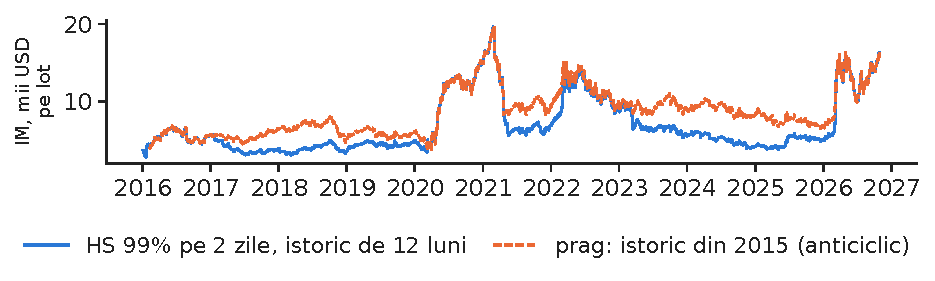
\includegraphics[width=\textwidth,height=0.480\textheight,keepaspectratio]{charts/ro/brent_im.pdf}\end{center}\vspace{-3mm}
\chartsource{Sursa: Yahoo Finance (contractul futures Brent ICE cu scadența cea mai apropiată, BZ=F); calcule proprii. Date: zile de tranzacționare 2016-01-01 - 2026-10-30; fără zilele de schimbare a contractului; 1 lot = 1.000 bbl.}
\vspace{0.5mm}
\begin{itemize}\setlength{\itemsep}{0pt}
  \item Prețul Brent a urcat de la 72{,}48 USD (27 februarie 2026) la 118{,}35 USD (31 martie 2026)
    \begin{itemize}\setlength{\itemsep}{0pt}
      \item IM cu 12 luni de date: 5\,970 $\to$ 16\,313 USD pe lot; cu pragul calculat din 2015: $\times$2{,}07 în loc de $\times$2{,}73
      \item Pierderi mai mari decît IM: 1{,}80\% din zile cu 12 luni de date, 0{,}66\% cu prag (ținta: 1\%)
    \end{itemize}
\end{itemize}
\par\vfill\manager{planificați lichiditățile pentru marja cerută într-o criză, nu pentru marja de astăzi.}\par\vspace{0.5mm}
\par\vfill\noindent{\scriptsize\color{FooterGray}(calcule proprii; RTS EMIR, art.~28; Brent ICE)}\hfill\qlink{EMQA\_L4\_brent\_im}{Quantlets/L4/EMQA_L4_brent_im}\par\vspace{0.5mm}
\end{frame}

\subsection{Garanții și limite}

\begin{frame}{Garanția pentru PZU se calculează din cuantila prognozată a prețului de mîine}
\footnotesize
\intuition{Ca să fie sigur că va cumpăra, furnizorul ofertează pînă la un preț ridicat; garanția acoperă acest preț înmulțit cu volumul.}
\begin{columns}[T,onlytextwidth]
\begin{column}{0.55\textwidth}
\[ G_t\ \ge\ Q\cdot 24\cdot \hat q_{\tau,t},\qquad \hat q_{\tau,t}=\beta_0+\beta_1P_{t-1}+\beta_2P_{t-7}+\textstyle\sum_j\delta_jD_{j,t} \]\[ \tilde q_{\tau,t}=\hat q_{\tau,t}+\hat c_t,\qquad \hat c_t=\hat q_\tau\big(P_s-\hat q_{\tau,s},\ s=t-365,\dots,t-1\big) \]{\footnotesize\begin{itemize}\setlength{\itemsep}{0pt}
  \item \textbf{\txtwhere}
    \begin{itemize}\setlength{\itemsep}{0pt}
      \item $G_t$ = garanția, EUR
      \item $\hat q_{\tau,t}$ = regresia cuantilică (QR) pe ultimele 365 de zile, ca la medierea prin regresie cuantilică (QRA), cursul 2
      \item $D_{j,t}$ = variabile pentru ziua săptămînii
      \item $\hat c_t$ = corecția conformală, din erorile trecute.
    \end{itemize}
\end{itemize}\par}
\end{column}
\begin{column}{0.42\textwidth}
\begin{itemize}\setlength{\itemsep}{1pt}
  \item \textbf{Pe datele din România}, $\tau$ = 0{,}99, 2017--2026
    \begin{itemize}\setlength{\itemsep}{0pt}
      \item Zile cu prețul sub prognoză: QR 96{,}90\%; QR lărgită 98{,}47\%; FHS 98{,}49\%
    \end{itemize}
  \item \textbf{Costul}, 100 MW în bandă
    \begin{itemize}\setlength{\itemsep}{0pt}
      \item În medie 0{,}371 milioane EUR pe zi; lărgirea costă +7{,}5\%
      \item 2017--2020: 0{,}172; 2021--2022: 0{,}649 milioane EUR pe zi
    \end{itemize}
\end{itemize}
\end{column}
\end{columns}
\par\vfill\manager{dimensionați linia bancară din spatele garanției pe cuantila din criză, înainte de criză.}\par\vspace{0.5mm}
\par\vfill\noindent{\scriptsize\color{FooterGray}(OPCOM, 2025; Koenker \& Bassett, 1978; Romano et al., 2019)}\hfill\tryit{notebook-ul Jupyter, secțiunea 6}\par\vspace{0.5mm}
\end{frame}

\begin{frame}{Lărgirea cozilor apropie cuantila de 99\% de acoperirea nominală}
\small
\begin{center}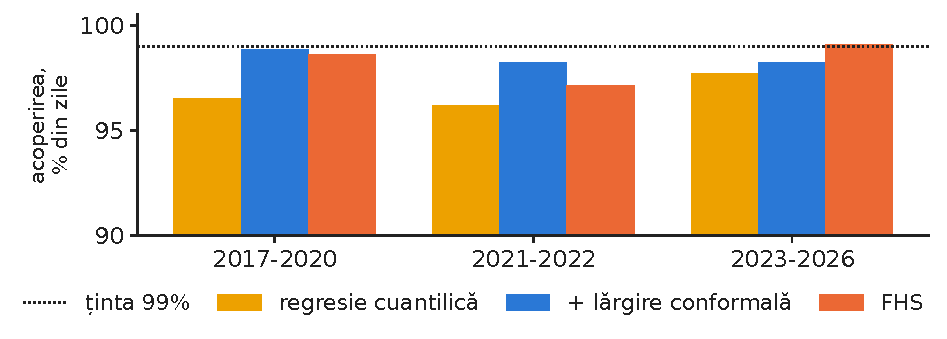
\includegraphics[width=\textwidth,height=0.500\textheight,keepaspectratio]{charts/ro/coverage.pdf}\end{center}\vspace{-3mm}
\chartsource{Sursa: energy-charts.info (Fraunhofer ISE); prețurile PZU ale OPCOM, prin ENTSO-E; estimări proprii. Date: prognoze 2017-01-01 - 2026-10-31, cuantila de 99\%.}
\vspace{0.5mm}
\begin{itemize}\setlength{\itemsep}{0pt}
  \item Testul Kupiec la 99\%: QR $<$0{,}001; QR lărgită 0{,}003; FHS 0{,}005
    \begin{itemize}\setlength{\itemsep}{0pt}
      \item La 95\%, QR lărgită trece testul ($p$ = 0{,}053), așa cum sugera cursul 2 pentru cozi
    \end{itemize}
\end{itemize}
\par\vfill\manager{o prognoză folosită pentru garanții trebuie să fie calibrată în coadă, nu doar precisă în medie.}\par\vspace{0.5mm}
\par\vfill\noindent{\scriptsize\color{FooterGray}(Nowotarski \& Weron, 2018, RSER; Romano et al., 2019)}\hfill\qlink{EMQA\_L4\_coverage}{Quantlets/L4/EMQA_L4_coverage}\par\vspace{0.5mm}
\end{frame}

\begin{frame}{Limita de poziție în MW trebuie să scadă atunci cînd VaR crește}
\footnotesize
\intuition{Conducerea stabilește un buget zilnic de risc, în EUR; biroul de tranzacționare îl împarte la VaR de azi pentru 1 MW.}
\begin{columns}[T,onlytextwidth]
\begin{column}{0.46\textwidth}
\[ Q^{\max}_t=\frac{B}{24\cdot\text{VaR}^{\text{FHS}}_{0{,}99,t}} \]{\footnotesize\begin{itemize}\setlength{\itemsep}{0pt}
  \item \textbf{\txtwhere}
    \begin{itemize}\setlength{\itemsep}{0pt}
      \item $B$ = bugetul zilnic de VaR, aici 250.000 EUR (o ipoteză de lucru)
      \item VaR în EUR/MWh
      \item $Q^{\max}_t$ = poziția deschisă maximă în bandă, în MW.
    \end{itemize}
\end{itemize}\par}
\end{column}
\begin{column}{0.51\textwidth}
\begin{itemize}\setlength{\itemsep}{1pt}
  \item \textbf{Pe datele din România}, VaR FHS de 99\%
    \begin{itemize}\setlength{\itemsep}{0pt}
      \item 2019 (mediana): VaR = 20{,}27 EUR/MWh; limita = 514 MW
      \item 12 iulie 2022: VaR = 245{,}80; limita = 42 MW
      \item 31 octombrie 2026: VaR = 53{,}15; limita = 196 MW
    \end{itemize}
  \item \textbf{De ce contează}
    \begin{itemize}\setlength{\itemsep}{0pt}
      \item O limită fixă în MW lasă suma expusă la risc să crească odată cu volatilitatea
      \item Un buget fix în EUR o menține constantă
    \end{itemize}
\end{itemize}
\end{column}
\end{columns}
\par\vfill\manager{stabiliți limitele în EUR de VaR și transformați-le zilnic în MW.}\par\vspace{0.5mm}
\par\vfill\noindent{\scriptsize\color{FooterGray}(estimări proprii)}\hfill\tryit{notebook-ul Jupyter, secțiunea 6}\par\vspace{0.5mm}
\end{frame}


\section{Riscul de preț pentru furnizori și producători}

\begin{frame}{Costul lunar la risc al unui furnizor, calculat cu repartiția normală}
\footnotesize
\intuition{Furnizorul stabilește prețul lunii viitoare după costul lunii curente; riscul este un salt al prețului ponderat cu consumul.}
\begin{columns}[T,onlytextwidth]
\begin{column}{0.52\textwidth}
\[ \bar P^{L}_m=\frac{\sum_h P_hL_h}{\sum_h L_h},\qquad o_m=\frac{\bar P^{L}_m}{\bar P^{L}_{m-1}}-1 \]\vspace{-2mm}\[ \text{CFaR}_{0{,}95}=\hat q_{0{,}95}(o_m) \]{\footnotesize\begin{itemize}\setlength{\itemsep}{0pt}
  \item \textbf{\txtwhere}
    \begin{itemize}\setlength{\itemsep}{0pt}
      \item $P_h$ = prețul orar
      \item $L_h$ = consumul național (profilul portofoliului)
      \item $o_m$ = depășirea costului
      \item Fluxul de numerar la risc (CFaR) = cuantila ei
      \item În EUR, pentru 100 MW în medie.
    \end{itemize}
\end{itemize}\par}
\end{column}
\begin{column}{0.45\textwidth}
\begin{itemize}\setlength{\itemsep}{1pt}
  \item \textbf{Pe datele din România}, 140 de luni, martie 2015 -- octombrie 2026
    \begin{itemize}\setlength{\itemsep}{0pt}
      \item Limita normală de 99\% (2015--2020): +50{,}5\%, depășită de 3 ori din 2021 (0{,}7 așteptate)
      \item Cea mai proastă lună, noiembrie 2024: +86{,}6\%, adică 5{,}96 milioane EUR
    \end{itemize}
  \item \textbf{Empiric, toate lunile}
    \begin{itemize}\setlength{\itemsep}{0pt}
      \item CFaR$_{0{,}95}$ = +39{,}9\%, adică 2{,}84 milioane EUR
      \item ES$_{0{,}95}$ = +60{,}2\%, adică 6{,}49 milioane EUR
    \end{itemize}
\end{itemize}
\end{column}
\end{columns}
\par\vfill\manager{includeți în oferta cu preț fix o primă calculată din ES sau acoperiți-o la termen (cursul 5).}\par\vspace{0.5mm}
\par\vfill\noindent{\scriptsize\color{FooterGray}(calcule proprii; tema 2)}\hfill\tryit{notebook-ul Jupyter, secțiunea 7}\par\vspace{0.5mm}
\end{frame}

\begin{frame}{Din 2021, limita lunară normală de 99\% a fost depășită de 3 ori (0{,}7 așteptate)}
\small
\begin{center}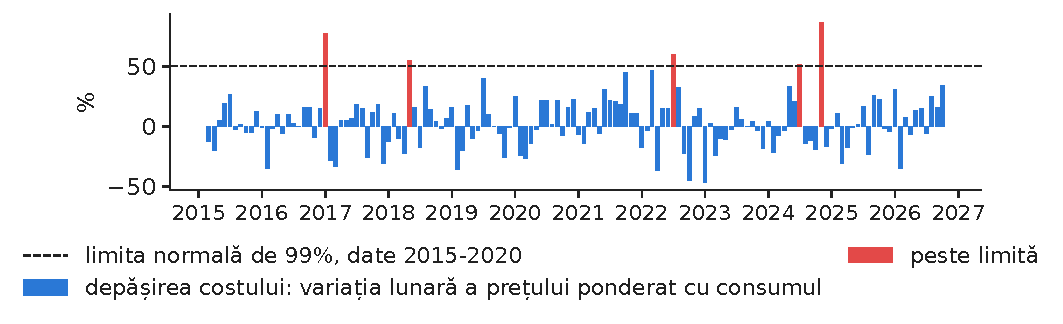
\includegraphics[width=\textwidth,height=0.520\textheight,keepaspectratio]{charts/ro/supplier_month.pdf}\end{center}\vspace{-3mm}
\chartsource{Sursa: energy-charts.info (Fraunhofer ISE); prețuri OPCOM; consumul ENTSO-E (date Transelectrica pentru România). Date: lunar, 2015-03 - 2026-10.}
\vspace{0.5mm}
\begin{itemize}\setlength{\itemsep}{0pt}
  \item Barele roșii depășesc limita calculată în 2020
    \begin{itemize}\setlength{\itemsep}{0pt}
      \item Cea mai mare depășire a apărut în noiembrie 2024, după vara anului 2024.
    \end{itemize}
\end{itemize}
\par\vfill\manager{reestimați limita lunară în fiecare trimestru și testați-o în condițiile lunilor din 2022.}\par\vspace{0.5mm}
\par\vfill\noindent{\scriptsize\color{FooterGray}(calcule proprii)}\hfill\qlink{EMQA\_L4\_supplier\_month}{Quantlets/L4/EMQA_L4_supplier_month}\par\vspace{0.5mm}
\end{frame}

\begin{frame}{Cozile pierderilor: coada furnizorului este mai groasă decît a producătorului}
\footnotesize
\intuition{Furnizorul pierde cînd prețul crește, producătorul cînd scade; prețurile sar mai mult în sus decît în jos.}
\begin{columns}[T,onlytextwidth]
\begin{column}{0.47\textwidth}
\[ L^{\text{cumpărător}}_t=+Q\,24\,X_t,\qquad L^{\text{vînzător}}_t=-Q\,24\,X_t \]{\footnotesize\begin{itemize}\setlength{\itemsep}{0pt}
  \item \textbf{\txtwhere}
    \begin{itemize}\setlength{\itemsep}{0pt}
      \item O singură repartiție a lui $X_t$, două cozi: superioară (furnizorul) și inferioară (producătorul care vinde pe piața spot)
      \item Asimetria lui $X_t$: 1{,}02.
    \end{itemize}
\end{itemize}\par}
\end{column}
\begin{column}{0.50\textwidth}
\begin{itemize}\setlength{\itemsep}{1pt}
  \item \textbf{Zilnic}, EUR/MWh, 1 ianuarie 2015 -- 31 octombrie 2026
    \begin{itemize}\setlength{\itemsep}{0pt}
      \item Cuantila de 99\% (furnizorul): +88{,}21; cuantila de 1\% (producătorul): \ensuremath{-}70{,}74
      \item ES$_{0{,}975}$: 91{,}29 (furnizorul) față de 74{,}92 (producătorul)
    \end{itemize}
  \item \textbf{Prețul de bază lunar}
    \begin{itemize}\setlength{\itemsep}{0pt}
      \item Cuantila de 95\% a variației: +42{,}4\%; cuantila de 5\%: \ensuremath{-}32{,}3\%
    \end{itemize}
\end{itemize}
\end{column}
\end{columns}
\par\vfill\manager{riscul de preț al producătorului este mai mic, dar un an secetos adaugă riscul de volum (diapozitivul următor).}\par\vspace{0.5mm}
\par\vfill\noindent{\scriptsize\color{FooterGray}(calcule proprii)}\hfill\tryit{notebook-ul Jupyter, secțiunea 7}\par\vspace{0.5mm}
\end{frame}

\begin{frame}{Studiul de caz C4: un indicator de risc sistemic și două riscuri specifice companiilor energetice}
\footnotesize
\begin{itemize}\setlength{\itemsep}{1pt}
  \item \textbf{Ce a făcut lucrarea} (Toma, Dima, Grecu, Pele \& Lessmann, 2026)
    \begin{itemize}\setlength{\itemsep}{0pt}
      \item Date și metodă: 100 de companii energetice europene, 2016--2026; regresii cuantilice de 5\% cu operatorul de contracție și selecție în normă absolută (LASSO); penalizarea medie este indicatorul de risc financiar al sectorului energetic (EFRM)
      \item Rezultat: EFRM surprinde șocurile din 2020 și 2022; împreună cu indicatorul compozit de stres sistemic al BCE (CISS), prognozează lunile volatile cu aria de sub curbă (AUC) 0,731
    \end{itemize}
  \item \textbf{Replicarea noastră} pe trei companii din România (OMV Petrom, Romgaz, Nuclearelectrica)
    \begin{itemize}\setlength{\itemsep}{0pt}
      \item AUC 0{,}38, față de 0{,}61 pentru volatilitatea trecută: un indicator sistemic are nevoie de multe companii, ca în lucrare
    \end{itemize}
  \item \textbf{Riscuri specifice energiei}
    \begin{itemize}\setlength{\itemsep}{0pt}
      \item Prima preț--volum a profilului casnic: 5{,}2\% din prețul de bază în 2025
      \item Recumpărarea în anul secetos pentru un parc hidro care a vîndut la termen producția mediană: 394 de milioane EUR (2022)
    \end{itemize}
\end{itemize}
\par\vfill\manager{includeți indicatorul sistemic, prima preț--volum și costul anului secetos în același tablou de bord.}\par\vspace{0.5mm}
\par\vfill\noindent{\scriptsize\color{FooterGray}(Toma, Dima, Grecu, Pele \& Lessmann, 2026, SSRN; studiul de caz C4)}\par\vspace{0.5mm}
\end{frame}

\begin{frame}{AIDA 2026: riscul sistemic din energia UE a crescut brusc din iulie 2021}
\footnotesize
\begin{itemize}\setlength{\itemsep}{1pt}
  \item \textbf{Ce a făcut lucrarea} (F.-M.\ Toma, conferința AIDA, 3 iunie 2026; lucrarea din studiul de caz C4)
    \begin{itemize}\setlength{\itemsep}{0pt}
      \item 100 de companii energetice europene, aprilie 2016 -- martie 2026: cuantila de 5\% a randamentului fiecărei firme, regresată prin LASSO pe celelalte 99 de firme, petrol, gaze și indici bursieri
      \item EFRM = penalizarea LASSO medie: mai multe legături necesare pentru a explica coada = expunere sistemică mai mare
    \end{itemize}
  \item \textbf{Ce a găsit}
    \begin{itemize}\setlength{\itemsep}{0pt}
      \item Rupturi ale EFRM: februarie 2020 (pandemia) și iulie 2021 (creșterea gazelor), cu șapte luni înaintea invaziei
      \item Riscul geopolitic a influențat EFRM abia după invazie: +1{,}52 puncte procentuale (model cu parametri variabili)
      \item Efectul asupra acțiunilor din Stoxx 600 s-a atenuat cu circa 60\%, cel asupra swapurilor pe riscul de credit pe 5 ani a rămas pozitiv
      \item Lunile volatile: AUC 0{,}731 pentru EFRM + CISS, 0{,}708 doar EFRM, 0{,}673 doar CISS
    \end{itemize}
\end{itemize}
\par\vspace{0.5mm}{\scriptsize \begin{itemize}\setlength{\itemsep}{0pt}
  \item Rezultatele sînt cele raportate de autori; prezentarea: \href{https://github.com/danpele/EMQA/blob/main/resources/aida2026/toma_energy_financial_risk_meter.pdf}{diapozitive}; lucrarea: \href{https://doi.org/10.2139/ssrn.6985301}{doi:10.2139/ssrn.6985301}.
\end{itemize}}
\par\vfill\manager{VaR proprie a unei firme nu vede contagiunea
    \begin{itemize}\setlength{\itemsep}{0pt}
      \item Urmăriți alături de ea un indicator sectorial.
    \end{itemize}}\par\vspace{0.5mm}
\par\vfill\noindent{\scriptsize\color{FooterGray}(Toma, AIDA, ASE, 3 iunie 2026; Toma, Dima, Grecu, Pele \& Lessmann, 2026, SSRN)}\par\vspace{0.5mm}
\end{frame}

\begin{frame}{AIDA 2026: riscul extrem al firmelor poluante anticipă prima de carbon}
\footnotesize
\begin{itemize}\setlength{\itemsep}{1pt}
  \item \textbf{Ce a făcut lucrarea} (prof.\ Wolfgang Karl Härdle, AIDA, 5 iunie 2026; cu R.\ Wang și L.\ Zhang)
    \begin{itemize}\setlength{\itemsep}{0pt}
      \item Puzzle-ul primei de carbon: cîștigă mai mult firmele poluante (risc) sau cele cu emisii reduse (preferințe verzi)?
      \item China, iul.\ 2014 -- feb.\ 2025: cîte 50 de firme poluante și cu emisii reduse; LASSO ca la EFRM, 63 de zile, cuantila de 5\%
      \item Indicatorul dinamic al riscului de carbon (CARDI) = indicatorul de risc financiar (FRM, $\lambda$ mediu), firme poluante / cu emisii reduse
    \end{itemize}
  \item \textbf{Ce a găsit}
    \begin{itemize}\setlength{\itemsep}{0pt}
      \item Regimurile de risc ridicat ale CARDI coincid cu evenimente neașteptate sau incipiente ale politicii climatice
      \item Creșterea CARDI anticipă o primă ajustată mai mare a firmelor cu emisii reduse luna următoare (0{,}022, 118 luni); raportul VaR condiționate nu
      \item Long pe firmele cu emisii reduse, short pe cele poluante doar cînd CARDI crește (2015--2024): 115{,}84\%, Sharpe 0{,}72 (permanent: 89{,}03\%, 0{,}49)
    \end{itemize}
  \item \textbf{Legătura cu acest curs}: EFRM din cadrul anterior, separat după intensitatea emisiilor
\end{itemize}
\par\vspace{0.5mm}{\scriptsize \begin{itemize}\setlength{\itemsep}{0pt}
  \item Rezultatele sînt cele raportate de autori; prezentarea: \href{https://github.com/danpele/EMQA/blob/main/resources/aida2026/wang_carbon_risk_dynamics.pdf}{diapozitive}; lucrarea: \href{https://doi.org/10.2139/ssrn.5757742}{doi:10.2139/ssrn.5757742}.
\end{itemize}}
\par\vfill\manager{într-o firmă de petrol și gaze, urmăriți CARDI: cînd crește, investitorii preferă firmele cu emisii reduse.}\par\vspace{0.5mm}
\par\vfill\noindent{\scriptsize\color{FooterGray}(Wang, Härdle \& Zhang, AIDA, ASE, 5 iunie 2026; 2025, SSRN)}\par\vspace{0.5mm}
\end{frame}


\section{Studiu de caz: creșterea prețurilor din toamna anului 2026}

\begin{frame}{Studiu de caz: în 2026 prețul s-a dublat treptat, fără salturi}
\small
\begin{center}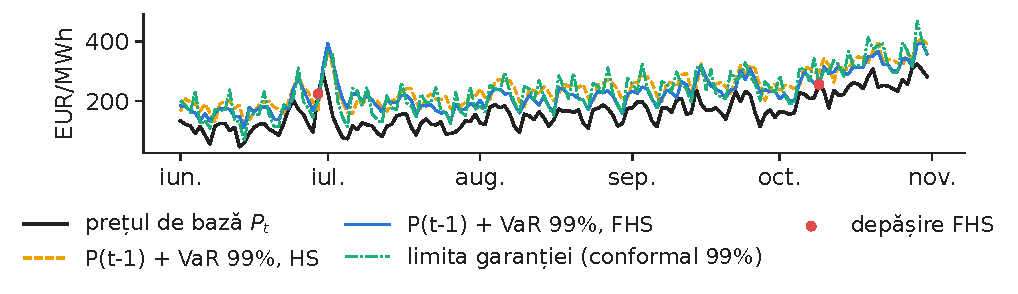
\includegraphics[width=\textwidth,height=0.472\textheight,keepaspectratio]{charts/ro/case2026.pdf}\end{center}\vspace{-3mm}
\chartsource{Sursa: energy-charts.info (Fraunhofer ISE); prețurile PZU ale OPCOM, prin ENTSO-E; estimări proprii. Date: date zilnice, 2026-06-01 - 2026-10-31.}
\vspace{0.5mm}
\begin{itemize}\setlength{\itemsep}{0pt}
  \item Media lunară: 122{,}99 EUR/MWh în iunie, 239{,}32 în octombrie; maximul: 323{,}76 EUR/MWh (29 octombrie 2026)
    \begin{itemize}\setlength{\itemsep}{0pt}
      \item Depășiri ale VaR de 99\% în 153 de zile (1{,}5 așteptate): FHS 2, HS 1, normală 3
    \end{itemize}
\end{itemize}
\par\vfill\manager{o creștere lentă trece testele VaR, dar consumă lichidități: urmăriți și nivelul prețului.}\par\vspace{0.5mm}
\par\vfill\noindent{\scriptsize\color{FooterGray}(estimări proprii; OPCOM)}\hfill\qlink{EMQA\_L4\_case2026}{Quantlets/L4/EMQA_L4_case2026}\par\vspace{0.5mm}
\end{frame}

\begin{frame}{Studiu de caz: riscul de piață și nevoia de lichidități în 2026}
\footnotesize
\begin{columns}[T,onlytextwidth]
\begin{column}{0.50\textwidth}
\begin{itemize}\setlength{\itemsep}{1pt}
  \item \textbf{Riscul de piață aproape nu s-a modificat}
    \begin{itemize}\setlength{\itemsep}{0pt}
      \item VaR FHS de 99\%: 61{,}64 EUR/MWh în iunie, 67{,}50 în octombrie
      \item Testul ES din 2023, FHS: $Z_2$ = \ensuremath{-}0{,}083, ipoteza nu este respinsă
    \end{itemize}
  \item \textbf{Nevoia de lichidități s-a dublat}
    \begin{itemize}\setlength{\itemsep}{0pt}
      \item Garanția pentru 100 MW pe piața pentru ziua următoare (cuantila de 99\% lărgită): 0{,}416 $\to$ 0{,}776 milioane EUR pe zi
      \item Zile cu prețul peste limita garanției: 3 (6 fără lărgire)
    \end{itemize}
\end{itemize}
\end{column}
\begin{column}{0.47\textwidth}
\begin{itemize}\setlength{\itemsep}{1pt}
  \item \textbf{Factura lunară a furnizorului}, 100 MW
    \begin{itemize}\setlength{\itemsep}{0pt}
      \item August: +25{,}1\% (2{,}38 milioane EUR); septembrie: +16{,}2\% (1{,}86); octombrie: +34{,}0\% (4{,}68)
      \item Fiecare lună sub limita de 99\% de +50{,}5\%, dar trei luni la rînd
    \end{itemize}
  \item \textbf{Factorii}
    \begin{itemize}\setlength{\itemsep}{0pt}
      \item Gazele TTF: 44{,}94 $\to$ 86{,}81 EUR/MWh (iunie $\to$ octombrie)
      \item Brent: 108{,}34 USD în octombrie; Germania--Luxemburg: 169{,}48 EUR/MWh
    \end{itemize}
\end{itemize}
\end{column}
\end{columns}
\par\vfill\manager{un raport de risc are nevoie, alături de VaR, de o secțiune de lichiditate: garanții, marje și depășirea cumulată a costului lunar.}\par\vspace{0.5mm}
\par\vfill\noindent{\scriptsize\color{FooterGray}(estimări proprii; OPCOM; Banca Mondială; Yahoo Finance)}\hfill\tryit{notebook-ul Jupyter, secțiunea 8}\par\vspace{0.5mm}
\end{frame}

\begin{frame}{Lista de verificare a biroului de risc pentru prețurile energiei}
\footnotesize
\begin{columns}[T,onlytextwidth]
\begin{column}{0.49\textwidth}
\begin{itemize}\setlength{\itemsep}{1pt}
  \item \textbf{Măsurarea}
    \begin{itemize}\setlength{\itemsep}{0pt}
      \item Definiți poziția și semnul pierderii (cumpărător sau vînzător)
      \item Folosiți numai datele cunoscute la închiderea licitației
      \item Raportați VaR și ES obținute prin două metode, dintre care una filtrată (FHS sau EVT)
    \end{itemize}
  \item \textbf{Verificarea}
    \begin{itemize}\setlength{\itemsep}{0pt}
      \item Testele Kupiec și Christoffersen și semaforul Basel pe mai mulți ani, inclusiv 2021--2022
      \item Testul $Z_2$ pentru ES; nu ierarhizați modelele pe baza cîtorva zile extreme
    \end{itemize}
\end{itemize}
\end{column}
\begin{column}{0.48\textwidth}
\begin{itemize}\setlength{\itemsep}{1pt}
  \item \textbf{Decizia}
    \begin{itemize}\setlength{\itemsep}{0pt}
      \item Limite exprimate în EUR de VaR, transformate zilnic în MW
      \item Garanții și linii de credit calculate din cuantile ridicate, bine calibrate
      \item O rezervă de lichidități pentru marja cerută într-o criză
    \end{itemize}
  \item \textbf{Raportarea}
    \begin{itemize}\setlength{\itemsep}{0pt}
      \item În EUR și în MW, lunar, cu lichiditatea alături de riscul de piață
    \end{itemize}
\end{itemize}
\end{column}
\end{columns}
\par\vfill\manager{tema 2 (sarcina 5) aplică această listă fluxului de numerar al rolului dumneavoastră.}\par\vspace{0.5mm}
\par\vfill\noindent{\scriptsize\color{FooterGray}(BCBS, 2019; RTS EMIR 153/2013; tema 2)}\par\vspace{0.5mm}
\end{frame}

\section*{Recapitulare}

\begin{frame}{Test 1: interpretarea VaR}
\small
\begin{itemize}
  \item VaR de 99\% pe o zi, pentru 100 MW, este de 162 de mii EUR
    \begin{itemize}\setlength{\itemsep}{0pt}
      \item Ce promite această cifră și ce nu spune?
    \end{itemize}
\end{itemize}
\vspace{2mm}
\begin{exampleblock}{R\u{a}spuns}
\begin{itemize}
  \item În aproximativ o zi din 100, pierderea ar trebui să o depășească
    \begin{itemize}\setlength{\itemsep}{0pt}
      \item Nu spune nimic despre mărimea pierderii în acele zile, pe care o măsoară ES (162 de mii EUR la 97{,}5\%).
    \end{itemize}
\end{itemize}
\end{exampleblock}
\end{frame}

\begin{frame}{Test 2: șapte depășiri}
\small
\begin{itemize}
  \item În ultimele 250 de zile, VaR de 99\% a fost depășită de 7 ori
    \begin{itemize}\setlength{\itemsep}{0pt}
      \item În ce zonă a semaforului se află modelul și ce arată testul Kupiec?
    \end{itemize}
\end{itemize}
\vspace{2mm}
\begin{exampleblock}{R\u{a}spuns}
\begin{itemize}
  \item Zona galbenă (5--9)
    \begin{itemize}\setlength{\itemsep}{0pt}
      \item LR$_{uc}$ = 5{,}50, $p$ = 0{,}019: ipoteza este respinsă la pragul de 5\%
      \item Recalibrați modelul (de exemplu, treceți de la HS la FHS) și continuați monitorizarea.
    \end{itemize}
\end{itemize}
\end{exampleblock}
\end{frame}

\begin{frame}{Test 3: zece zile}
\small
\begin{itemize}
  \item Directorul financiar calculează VaR pe 10 zile ca $\sqrt{10}$ înmulțit cu VaR pe o zi
    \begin{itemize}\setlength{\itemsep}{0pt}
      \item Este o abordare prudentă sau risipitoare pentru energie?
    \end{itemize}
\end{itemize}
\vspace{2mm}
\begin{exampleblock}{R\u{a}spuns}
\begin{itemize}
  \item Risipitoare: prețurile energiei revin spre medie, iar cuantila empirică de 99\% pe 10 zile este doar de 1{,}72 ori cea pe o zi în România, nu de 3{,}16 ori.
\end{itemize}
\end{exampleblock}
\end{frame}

\begin{frame}{Test 4: un apel în marjă}
\small
\begin{itemize}
  \item Ați vîndut 100 de loturi Brent pentru a vă acoperi producția
    \begin{itemize}\setlength{\itemsep}{0pt}
      \item Astăzi prețul crește cu 5 USD pe baril
      \item Ce se întîmplă diseară?
    \end{itemize}
\end{itemize}
\vspace{2mm}
\begin{exampleblock}{R\u{a}spuns}
\begin{itemize}
  \item Plătiți o marjă de variație de 100 $\times$ 1.000 $\times$ 5 = 500.000 USD în numerar
    \begin{itemize}\setlength{\itemsep}{0pt}
      \item Țițeiul pe care îl veți vinde mai tîrziu valorează mai mult, dar banii pleacă astăzi.
    \end{itemize}
\end{itemize}
\end{exampleblock}
\end{frame}

\begin{frame}{Test 5: o garanție prea mică}
\small
\begin{itemize}
  \item Prognoza dumneavoastră pentru cuantila de 99\% a prețului de mîine a fost depășită în 111 zile din 3\,585
    \begin{itemize}\setlength{\itemsep}{0pt}
      \item Ce faceți?
    \end{itemize}
\end{itemize}
\vspace{2mm}
\begin{exampleblock}{R\u{a}spuns}
\begin{itemize}
  \item Lărgiți coada cu o corecție conformală calculată din erorile recente: acoperirea crește de la 96{,}90\% la 98{,}47\%, cu o garanție mai mare cu doar 7{,}5\%.
\end{itemize}
\end{exampleblock}
\end{frame}

\begin{frame}{Recapitulare}
\small
\vspace{-2mm}\begin{multicols}{2}\scriptsize\tableofcontents\end{multicols}
\begin{itemize}\setlength{\itemsep}{1pt}
  \item VaR este o cuantilă, iar ES media pierderilor de dincolo de ea
    \begin{itemize}\setlength{\itemsep}{0pt}
      \item Pe prețurile energiei, repartiția normală eșuează, metodele filtrate (FHS, EVT) se apropie cel mai mult de țintă și niciuna nu a fost corectă în 2021--2022.
    \end{itemize}
  \item Aceleași cuantile stabilesc limite, marje și garanții
    \begin{itemize}\setlength{\itemsep}{0pt}
      \item Studiul de caz din 2026 arată că lichiditatea, nu VaR, este prima afectată
      \item Cursul următor: acoperirea riscului cu instrumente derivate (cursul 5).
    \end{itemize}
\end{itemize}
\end{frame}

\begin{frame}{Cercetările grupului nostru despre riscul pe piețele de energie}
\footnotesize
\begin{itemize}\setlength{\itemsep}{1pt}
  \item \textbf{Indicatorul de risc financiar al sectorului energetic} (Toma, Dima, Grecu, Pele \& Lessmann, 2026, SSRN)
    \begin{itemize}\setlength{\itemsep}{0pt}
      \item Ce a făcut lucrarea: a construit un indicator de risc sistemic pentru sectorul energetic din UE, din regresii cuantilice LASSO pe 100 de companii; rezultat: indicatorul surprinde șocurile din 2020 și 2022 (studiul de caz C4)
    \end{itemize}
  \item \textbf{Modele fundaționale pentru VaR și ES} (Jheng, Tak, Găman, Mazurencu-Marinescu-Pele \& Pele, 2026)
    \begin{itemize}\setlength{\itemsep}{0pt}
      \item Date: zece serii de randamente zilnice din cinci piețe din Europa Centrală și de Est (CEE), inclusiv România, cu evaluare în afara eșantionului în 2018--2025
      \item Metodă: trei modele preantrenate pentru serii de timp, folosite fără reantrenare, comparate cu metode clasice; testele Kupiec, Christoffersen, Acerbi--Székely și semaforul Basel
      \item Rezultat: 90\% din ferestre în zona verde pentru cel mai bun model neajustat și 96{,}7\% după o calibrare conformală glisantă, cel mai bun rezultat dintre toate
    \end{itemize}
  \item \textbf{Cît de precisă este o comparație a prognozelor ES?} (Pele \& Mazurencu-Marinescu-Pele, 2026, Mathematics)
    \begin{itemize}\setlength{\itemsep}{0pt}
      \item Ce a făcut lucrarea: a transformat limita de precizie $(n\alpha)^{-1/2}$ a ES în patru diagnostice practice, inclusiv o regulă pentru mărimea eșantionului
      \item Rezultat: pe active financiare globale, aproximativ una din cinci comparații între prognoze ES nu este concludentă la nivelurile de risc cerute de reglementare
    \end{itemize}
\end{itemize}
\par\vspace{0.5mm}{\scriptsize \begin{itemize}\setlength{\itemsep}{0pt}
  \item Rezultatele de pe acest diapozitiv sînt cele raportate în lucrări; celelalte cifre din curs provin din calculele noastre.
\end{itemize}}
\par\vfill\noindent{\scriptsize\color{FooterGray}(Academia de Studii Economice din București; Academia Română, Institutul de Prognoză Economică)}\par\vspace{0.5mm}
\end{frame}

\begin{frame}{Lecturi și resurse suplimentare}
\small
\begin{columns}[T,onlytextwidth]
\begin{column}{0.52\textwidth}
\begin{itemize}\setlength{\itemsep}{1pt}
  \item \textbf{McNeil, Frey \& Embrechts}, \textit{Quantitative Risk Management}, ed.\ a 2-a: VaR, ES, EVT, testare retrospectivă.
  \item \textbf{Christoffersen}, \textit{Elements of Financial Risk Management}, ed.\ a 2-a: FHS și testare retrospectivă, cu exerciții.
  \item \textbf{BCE}, Financial stability risks from energy derivatives markets (2022): \href{https://www.ecb.europa.eu/pub/financial-stability/fsr/special/html/ecb.fsrart202211_01~173476301a.en.html}{ecb.europa.eu}.
\end{itemize}
\end{column}
\begin{column}{0.45\textwidth}
\begin{itemize}\setlength{\itemsep}{1pt}
  \item \textbf{Acest curs}: cod, date, notebook-uri Jupyter --- \href{https://github.com/danpele/EMQA}{github.com/danpele/EMQA}.
  \item \textbf{Tema 2}, sarcina 5: VaR și ES ale fluxului de numerar al rolului dumneavoastră, cu testare retrospectivă.
  \item \textbf{OPCOM}, procedura privind garanțiile pentru PZU: \href{https://www.opcom.ro}{opcom.ro}.
  \item \textbf{Exercițiu practic}: notebook-ul Jupyter reproduce toate graficele și cifrele din acest curs --- \href{\emqarepo/\emqanb}{notebooks/}.
\end{itemize}
\end{column}
\end{columns}
\end{frame}

\begin{frame}{Bibliografie (1/4)}
\scriptsize
\begin{itemize}\setlength{\itemsep}{1pt}\scriptsize
\item Acerbi, C.\ \& Székely, B.\ (2014). Backtesting expected shortfall. \textit{Risk}, 27(11), 76--81. \href{https://www.risk.net/risk-magazine/technical-paper/2381658/back-testing-expected-shortfall}{risk.net}
\item Acerbi, C.\ \& Tasche, D.\ (2002). On the coherence of expected shortfall. \textit{Journal of Banking \& Finance}, 26(7), 1487--1503. \href{https://doi.org/10.1016/S0378-4266(02)00283-2}{doi:10.1016/S0378-4266(02)00283-2}
\item Artzner, P., Delbaen, F., Eber, J.-M.\ \& Heath, D.\ (1999). Coherent measures of risk. \textit{Mathematical Finance}, 9(3), 203--228. \href{https://doi.org/10.1111/1467-9965.00068}{doi:10.1111/1467-9965.00068}
\item Balkema, A.\,A.\ \& de Haan, L.\ (1974). Residual life time at great age. \textit{Annals of Probability}, 2(5), 792--804. \href{https://doi.org/10.1214/aop/1176996548}{doi:10.1214/aop/1176996548}
\item Barone-Adesi, G., Giannopoulos, K.\ \& Vosper, L.\ (1999). VaR without correlations for portfolios of derivative securities. \textit{Journal of Futures Markets}, 19(5), 583--602. \href{https://doi.org/10.1002/(SICI)1096-9934(199908)19:5\%3C583::AID-FUT5\%3E3.0.CO;2-S}{doi.org (Wiley)}
\item BCBS (1996). Supervisory framework for the use of ``backtesting'' in conjunction with the internal models approach to market risk capital requirements. Basel Committee on Banking Supervision, January 1996. \href{https://www.bis.org/publ/bcbs22.htm}{bis.org/publ/bcbs22.htm}
\item BCBS (2019). Minimum capital requirements for market risk. Basel Committee on Banking Supervision, January 2019. \href{https://www.bis.org/bcbs/publ/d457.htm}{bis.org/bcbs/publ/d457.htm}
\item Bollerslev, T.\ (1986). Generalized autoregressive conditional heteroskedasticity. \textit{Journal of Econometrics}, 31(3), 307--327. \href{https://doi.org/10.1016/0304-4076(86)90063-1}{doi:10.1016/0304-4076(86)90063-1}
\item Chan, K.\,F.\ \& Gray, P.\ (2006). Using extreme value theory to measure value-at-risk for daily electricity spot prices. \textit{International Journal of Forecasting}, 22(2), 283--300. \href{https://doi.org/10.1016/j.ijforecast.2005.10.002}{doi:10.1016/j.ijforecast.2005.10.002}
\end{itemize}
\end{frame}

\begin{frame}{Bibliografie (2/4)}
\scriptsize
\begin{itemize}\setlength{\itemsep}{1pt}\scriptsize
\item Christoffersen, P.\,F.\ (1998). Evaluating interval forecasts. \textit{International Economic Review}, 39(4), 841--862. \href{https://doi.org/10.2307/2527341}{doi:10.2307/2527341}
\item Christoffersen, P.\,F.\ (2012). \textit{Elements of Financial Risk Management}, 2nd ed. Academic Press. \href{https://shop.elsevier.com/books/elements-of-financial-risk-management/christoffersen/978-0-12-374448-7}{elsevier.com}
\item Commission Delegated Regulation (EU) No 153/2013 of 19 December 2012 on requirements for central counterparties (RTS under EMIR), \textit{Official Journal of the EU}, L 52, 23.2.2013, Art.~24--28. \href{https://eur-lex.europa.eu/eli/reg_del/2013/153/oj}{eur-lex.europa.eu/eli/reg\_del/2013/153/oj}
\item Commission Delegated Regulation (EU) 2022/2311 of 21 October 2022 as regards temporary emergency measures on collateral requirements. \textit{Official Journal of the EU}, L 307, 28.11.2022. \href{https://eur-lex.europa.eu/eli/reg_del/2022/2311/oj}{eur-lex.europa.eu/eli/reg\_del/2022/2311/oj}
\item ECB --- Furtuna, O., Grassi, A., Ianiro, A., Kallage, K., Koci, R., Lenoci, F., Sowiński, A.\ \& Vacirca, F.\ (2022). Financial stability risks from energy derivatives markets. \textit{Financial Stability Review}, European Central Bank, November 2022. \href{https://www.ecb.europa.eu/press/financial-stability-publications/fsr/special/html/ecb.fsrart202211_01~173476301a.en.html}{ecb.europa.eu}
\item Gneiting, T.\ (2011). Making and evaluating point forecasts. \textit{Journal of the American Statistical Association}, 106(494), 746--762. \href{https://doi.org/10.1198/jasa.2011.r10138}{doi:10.1198/jasa.2011.r10138}
\item Jheng, S.-L., Tak, R., Găman, Ș., Mazurencu-Marinescu-Pele, M.\ \& Pele, D.\,T.\ (2026). Can foundation models manage risk? Zero-shot VaR and ES forecasting with conformal calibration in CEE markets. \textit{Economic Computation and Economic Cybernetics Studies and Research}, 60(2), 267--290. \href{https://doi.org/10.24818/18423264/60.2.26.14}{doi:10.24818/18423264/60.2.26.14}
\item Jorion, P.\ (2007). \textit{Value at Risk: The New Benchmark for Managing Financial Risk}, 3rd ed. McGraw-Hill. \href{https://www.mheducation.com.au/ebook-value-at-risk-the-new-benchmark-for-managing-financial-risk-3e-9781307199963-aus}{mheducation.com.au}
\end{itemize}
\end{frame}

\begin{frame}{Bibliografie (3/4)}
\scriptsize
\begin{itemize}\setlength{\itemsep}{1pt}\scriptsize
\item Koenker, R.\ \& Bassett, G.\ (1978). Regression quantiles. \textit{Econometrica}, 46(1), 33--50. \href{https://doi.org/10.2307/1913643}{doi:10.2307/1913643}
\item Kupiec, P.\,H.\ (1995). Techniques for verifying the accuracy of risk measurement models. \textit{Journal of Derivatives}, 3(2), 73--84. \href{https://doi.org/10.3905/jod.1995.407942}{doi:10.3905/jod.1995.407942}
\item McNeil, A.\,J.\ \& Frey, R.\ (2000). Estimation of tail-related risk measures for heteroscedastic financial time series: An extreme value approach. \textit{Journal of Empirical Finance}, 7(3--4), 271--300. \href{https://doi.org/10.1016/S0927-5398(00)00012-8}{doi:10.1016/S0927-5398(00)00012-8}
\item McNeil, A.\,J., Frey, R.\ \& Embrechts, P.\ (2015). \textit{Quantitative Risk Management: Concepts, Techniques and Tools}, revised ed. Princeton University Press. \href{https://press.princeton.edu/books/hardcover/9780691166278/quantitative-risk-management}{press.princeton.edu}
\item Nowotarski, J.\ \& Weron, R.\ (2018). Recent advances in electricity price forecasting: A review of probabilistic forecasting. \textit{Renewable and Sustainable Energy Reviews}, 81, 1548--1568. \href{https://doi.org/10.1016/j.rser.2017.05.234}{doi:10.1016/j.rser.2017.05.234}
\item OPCOM (2025). Procedura privind constituirea, verificarea și utilizarea garanțiilor financiare pentru participarea la Piața pentru Ziua Următoare, rev.\ 10, May 2025. \href{https://www.opcom.ro}{opcom.ro}
\item Pele, D.\,T.\ \& Mazurencu-Marinescu-Pele, M.\ (2026). Finite-sample precision limits for expected shortfall forecast comparisons. \textit{Mathematics}, 14(13), 2316. \href{https://doi.org/10.3390/math14132316}{doi:10.3390/math14132316}
\item Pele, D.\,T., Bolovăneanu, V., Ginavar, A.\,T., Lessmann, S.\ \& Härdle, W.\,K.\ (2026). Recalibrating tail risk forecasts under temporal dependence: conformal audit of foundation models for VaR forecasting. AIDA Conference, Bucharest University of Economic Studies, 4 June 2026. \href{https://github.com/danpele/EMQA/blob/main/resources/aida2026/pele_conformal_tail_risk.pdf}{github.com/danpele/EMQA/resources/aida2026}
\end{itemize}
\end{frame}

\begin{frame}{Bibliografie (4/4)}
\scriptsize
\begin{itemize}\setlength{\itemsep}{1pt}\scriptsize
\item Pickands, J.\ (1975). Statistical inference using extreme order statistics. \textit{Annals of Statistics}, 3(1), 119--131. \href{https://doi.org/10.1214/aos/1176343003}{doi:10.1214/aos/1176343003}
\item Romano, Y., Patterson, E.\ \& Candès, E.\ (2019). Conformalized quantile regression. \textit{Advances in Neural Information Processing Systems}, 32, 3543--3553. \href{https://proceedings.neurips.cc/paper/2019/hash/5103c3584b063c431bd1268e9b5e76fb-Abstract.html}{proceedings.neurips.cc}
\item Toma, F.-M., Dima, D.-M., Grecu, R., Pele, D.\,T.\ \& Lessmann, S.\ (2026). Energy Financial Risk Meter: Systemic risk in the EU energy sector. SSRN Working Paper 6985301. \href{https://doi.org/10.2139/ssrn.6985301}{doi:10.2139/ssrn.6985301}
\item Toma, F.-M.\ (2026). Energy Financial Risk Meter: systemic risk in the EU energy sector (with D.-M.\ Dima, R.\ Grecu, D.\,T.\ Pele and S.\ Lessmann). AIDA Conference, Bucharest University of Economic Studies, 3 June 2026. \href{https://github.com/danpele/EMQA/blob/main/resources/aida2026/toma_energy_financial_risk_meter.pdf}{github.com/danpele/EMQA/resources/aida2026}
\item Wang, R., Härdle, W.\,K.\ \& Zhang, L.\ (2025). Measuring carbon risk dynamics. SSRN Working Paper 5757742. \href{https://doi.org/10.2139/ssrn.5757742}{doi:10.2139/ssrn.5757742}
\item Wang, R., Härdle, W.\,K.\ \& Zhang, L.\ (2026). Measuring carbon risk dynamics. AIDA Conference, Bucharest University of Economic Studies, 5 June 2026. \href{https://github.com/danpele/EMQA/blob/main/resources/aida2026/wang_carbon_risk_dynamics.pdf}{github.com/danpele/EMQA/resources/aida2026}
\item Weron, R.\ (2014). Electricity price forecasting: A review of the state-of-the-art with a look into the future. \textit{International Journal of Forecasting}, 30(4), 1030--1081. \href{https://doi.org/10.1016/j.ijforecast.2014.08.008}{doi:10.1016/j.ijforecast.2014.08.008}
\end{itemize}
\end{frame}

\appendix

\section*{Anexă}

\begin{frame}{Anexa A: ES pentru repartițiile normală și Student-$t$}
\small
\begin{columns}[T,onlytextwidth]
\begin{column}{0.49\textwidth}
\[ \text{ES}^{N}_\alpha=\frac{1}{1-\alpha}\int_{z_\alpha}^{\infty}(\mu+\sigma z)\varphi(z)\,dz=\mu+\sigma\frac{\varphi(z_\alpha)}{1-\alpha} \]\begin{itemize}\setlength{\itemsep}{1pt}
  \item Deoarece $\int_{c}^{\infty}z\varphi(z)\,dz=\varphi(c)$ (derivata lui $\varphi$ este $-z\varphi$).
  \item La $\alpha$ = 0{,}975, ES$^N$ = $\mu$ + 2{,}338$\sigma$, aproape egal cu VaR$^N_{0{,}99}$ = $\mu$ + 2{,}326$\sigma$: de aceea FRTB a înlocuit o măsură cu cealaltă.
\end{itemize}
\end{column}
\begin{column}{0.48\textwidth}
\[ \text{ES}^{t}_\alpha=m+s\,\frac{g_\nu(t_{\nu,\alpha})}{1-\alpha}\cdot\frac{\nu+t_{\nu,\alpha}^{2}}{\nu-1},\quad \nu>1 \]\begin{itemize}\setlength{\itemsep}{1pt}
  \item Din $\int_c^\infty x\,g_\nu(x)\,dx=g_\nu(c)\,(\nu+c^2)/(\nu-1)$
    \begin{itemize}\setlength{\itemsep}{0pt}
      \item Pentru $\nu\le 1$ media, deci și ES, nu există.
    \end{itemize}
  \item Estimăm zilnic $(m,s,\nu)$ prin MLE
    \begin{itemize}\setlength{\itemsep}{0pt}
      \item $\nu$ este menținut cel puțin la 2{,}2, pentru ca varianța să existe.
    \end{itemize}
\end{itemize}
\end{column}
\end{columns}
\par\vfill\noindent{\scriptsize\color{FooterGray}(McNeil, Frey \& Embrechts, 2015, ch.~2)}\par\vspace{0.5mm}
\end{frame}

\begin{frame}{Anexa B: VaR și ES din coada Pareto generalizată}
\small
\begin{columns}[T,onlytextwidth]
\begin{column}{0.50\textwidth}
\[ \Pr(Z>z)\approx\frac{N_u}{n}\Big(1+\xi\frac{z-u}{\beta}\Big)^{-1/\xi},\quad z>u \]\[ \Pr(Z>\text{VaR}_\alpha)=1-\alpha\ \Rightarrow \]\vspace{-2mm}\[ \text{VaR}_\alpha=u+\frac{\beta}{\xi}\Big[\Big(\frac{n(1-\alpha)}{N_u}\Big)^{-\xi}-1\Big] \]\begin{itemize}\setlength{\itemsep}{1pt}
  \item Teorema Pickands--Balkema--de Haan: pentru un prag $u$ ridicat, excesele peste $u$ urmează aproximativ o repartiție GPD, pentru aproape orice repartiție.
\end{itemize}
\end{column}
\begin{column}{0.47\textwidth}
\[ \E[Z-v\mid Z>v]=\frac{\beta+\xi(v-u)}{1-\xi} \]\vspace{-2mm}\[ \Rightarrow\ \text{ES}_\alpha=\frac{\text{VaR}_\alpha+\beta-\xi u}{1-\xi} \]\begin{itemize}\setlength{\itemsep}{1pt}
  \item Excesul mediu este liniar în $v$ pentru GPD (cu condiția $\xi<1$)
    \begin{itemize}\setlength{\itemsep}{0pt}
      \item $\xi>0$ = coadă groasă, $\xi=0$ = coadă exponențială, $\xi<0$ = coadă mărginită.
    \end{itemize}
  \item EVT condiționată: aplicăm formula lui $z_t=e_t/\sigma_t$, apoi VaR$_t=\mu_{d(t)}+\sigma_t\,$VaR$^z_\alpha$.
\end{itemize}
\end{column}
\end{columns}
\par\vfill\noindent{\scriptsize\color{FooterGray}(Pickands, 1975; Balkema \& de Haan, 1974; McNeil \& Frey, 2000)}\par\vspace{0.5mm}
\end{frame}

\begin{frame}{Anexa C: cele trei teste retrospective, în detaliu}
\footnotesize
\begin{columns}[T,onlytextwidth]
\begin{column}{0.49\textwidth}
\begin{itemize}\setlength{\itemsep}{1pt}
  \item \textbf{Kupiec și Christoffersen}
    \begin{itemize}\setlength{\itemsep}{0pt}
      \item În ipoteza $H_0$, fiecare $I_t$ este o variabilă Bernoulli($p$), independentă; LR$_{uc}$ compară $p$ cu $\hat p$
      \item LR$_{ind}$ compară un lanț Markov de ordinul întîi cu ipoteza de independență; LR$_{cc}$ = LR$_{uc}$ + LR$_{ind}\sim\chi^2_2$, valoarea critică la 5\%: 5{,}99
    \end{itemize}
  \item \textbf{Semaforul Basel}
    \begin{itemize}\setlength{\itemsep}{0pt}
      \item $x\sim$ Binomial(250; 0{,}01) pentru un model corect
      \item $\Pr(x\le4)$ = 89{,}22\%, $\Pr(5\le x\le9)$ = 10{,}76\%, $\Pr(x\ge10)$ = 0{,}025\%
    \end{itemize}
\end{itemize}
\end{column}
\begin{column}{0.48\textwidth}
\begin{itemize}\setlength{\itemsep}{1pt}
  \item \textbf{Testul Acerbi--Székely $Z_2$}
    \begin{itemize}\setlength{\itemsep}{0pt}
      \item Deoarece $\E[L_tI_t]=(1-\alpha)\text{ES}_t$ atunci cînd VaR și ES sînt corecte, $\E[Z_2]=0$
      \item $Z_2$ combină o eroare de VaR (numărul greșit de $I_t$) cu o eroare de ES (mărimea greșită); ES nu este elicitabil, de aceea se testează împreună cu VaR
      \item Valoarea $p$: 2.000 de traiectorii simulate, fiecare zi fiind extrasă din repartiția prognozată de modelul respectiv (HS: fereastra; FHS: $\mu+\sigma z^*$; EVT: GPD peste $u$)
    \end{itemize}
\end{itemize}
\end{column}
\end{columns}
\par\vfill\noindent{\scriptsize\color{FooterGray}(Kupiec, 1995; Christoffersen, 1998; BCBS, 1996; Acerbi \& Székely, 2014)}\par\vspace{0.5mm}
\end{frame}

\begin{frame}{Anexa D: aceeași testare retrospectivă pentru Germania--Luxemburg}
\small
\begin{center}{\footnotesize\renewcommand{\arraystretch}{1.2}\setlength{\tabcolsep}{4pt}
\begin{tabular}{@{}lrrrrrrrrr@{}}\toprule
DE-LU & 95\%: proporția & Kupiec $p$ & 99\%: număr & proporția & Kupiec $p$ & Chr.\ $p$ & roșu, \% & $Z_2$ & $p$ \\ \midrule
HS & 6{,}38 & $<$0{,}001 & 60 & 1{,}67 & $<$0{,}001 & 0{,}998 & 9{,}2 & 0{,}529 & $<$0{,}001 \\
Normală & 6{,}66 & $<$0{,}001 & 107 & 2{,}98 & $<$0{,}001 & 0{,}332 & 16{,}3 & 1{,}250 & $<$0{,}001 \\
Student-$t$ & 8{,}33 & $<$0{,}001 & 67 & 1{,}87 & $<$0{,}001 & 0{,}174 & 9{,}0 & 0{,}617 & 0{,}001 \\
FHS & 5{,}82 & 0{,}028 & 58 & 1{,}62 & $<$0{,}001 & 0{,}948 & 2{,}7 & 0{,}305 & 0{,}009 \\
EVT & 5{,}93 & 0{,}013 & 53 & 1{,}48 & 0{,}007 & 0{,}811 & 0{,}7 & 0{,}283 & 0{,}007 \\
\bottomrule\end{tabular}}\end{center}
\par\vspace{0.5mm}{\scriptsize \begin{itemize}\setlength{\itemsep}{0pt}
  \item Testare retrospectivă 1 ianuarie 2017 -- 31 octombrie 2026, 3\,591 de zile; aceleași metode și ferestre ca pentru România.
  \item Clasamentul este același ca în România: repartiția normală are cele mai slabe rezultate, metodele filtrate cele mai bune.
\end{itemize}}
\par\vfill\noindent{\scriptsize\color{FooterGray}(estimări proprii; EPEX SPOT)}\par\vspace{0.5mm}
\end{frame}

\end{document}
